%If on Overleaf, first compile file "externalize-tikz.tex" in folder "images". Then compile "report.tex"
%This saves the images as pdf in the cache and it optimises the compilation time
\documentclass{report}
\usepackage[utf8]{inputenc}
\usepackage[T1]{fontenc}
\usepackage[english]{babel}
\usepackage{amsmath}
\usepackage{amssymb}
\usepackage{mathtools}
\usepackage{enumerate}
\usepackage{enumitem}
\usepackage{amsthm}
\usepackage[colorlinks=true,linkcolor=blue]{hyperref}
\usepackage{graphicx}
\usepackage{subcaption}
\usepackage{tikz-cd}
\usepackage{pgfplots}
\pgfplotsset{compat=1.15}
\usepackage{stmaryrd}
\SetSymbolFont{stmry}{bold}{U}{stmry}{m}{n}
\usepackage[backend=biber,style=alphabetic]{biblatex}
\addbibresource{bibliography.bib}
\usepackage{csquotes}
\usepackage[left=2cm,top=2.5cm,right=1.5cm,bottom=2.5cm]{geometry}
\setlength{\parindent}{0pt}
\renewcommand{\baselinestretch}{1.1}

\DeclareMathOperator{\Spf}{Spf}
\DeclareMathOperator{\Spec}{Spec}
\DeclareMathOperator{\Proj}{Proj}
\DeclareMathOperator{\Mod}{Mod}
\DeclareMathOperator{\Top}{Top}
\DeclareMathOperator{\id}{id}
\DeclareMathOperator{\PSh}{PSh}
\DeclareMathOperator{\Sh}{Sh}
\DeclareMathOperator{\Et}{\acute{E}t}
\DeclareMathOperator{\Cat}{Cat}
\DeclareMathOperator{\Hom}{Hom}
\DeclareMathOperator{\im}{im}
\DeclareMathOperator{\Alg}{Alg}
\DeclareMathOperator{\Art}{Art}
\DeclareMathOperator{\Ab}{Ab}
\DeclareMathOperator{\chara}{char}
\DeclareMathOperator{\Pic}{Pic}
\DeclareMathOperator{\Br}{Br}
\DeclareMathOperator{\I}{I}
\DeclareMathOperator{\II}{II}
\DeclareMathOperator{\III}{III}
\DeclareMathOperator{\IV}{IV}
\DeclareMathOperator{\Sch}{Sch}
\DeclareMathOperator{\Div}{Div}
\DeclareMathOperator{\NS}{NS}
\DeclareMathOperator{\Num}{Num}

%\renewcommand{\thechapter}{\Roman{chapter}}

\newtheorem{theorem}[equation]{Theorem}
\newtheorem{corollary}[equation]{Corollary}
\newtheorem{proposition}[equation]{Proposition}
\newtheorem{lemma}[equation]{Lemma}
\theoremstyle{definition}
\newtheorem{definition}[equation]{Definition}
\newtheorem{remark}[equation]{Remark}
\newtheorem{example}[equation]{Example}

\title{Formal group laws arising from algebraic varieties}
\author{Alejandro Plaza Gall\'{a}n\\\\Advisor:\\Christian Liedtke}
\date{15 June 2024}

\begin{document}
\maketitle

\tableofcontents
\newpage

\chapter{Elliptic surfaces}

In this work, we want to study the formal Brauer group over elliptic surfaces. Restricting us to these particular varieties will let us relate some properties of the formal Brauer group with coefficients that define the elliptic surfaces. We will treat the algebraic varieties as schemes, this is, locally ringed spaces that are locally the spectrum of a ring. For more information about algebraic varieties and schemes, see \cite{hartshorne1977algebraic}.

\section{Elliptic curves}

Hartshorne \cite[Section~IV.4]{hartshorne1977algebraic} gives the theory of elliptic curves over an algebraically closed field. Let's start from the beginning, by defining what we mean with elliptic curve.

\begin{definition}
A curve $X$ is an integral smooth projective and separated scheme of dimension $1$ of finite type over a field $k$.
\end{definition}

\begin{definition}
An elliptic curve is a pair $(X,P_0)$ consisting of a curve $X$ over $k$ of genus $1$, together with a rational point $P_0\in X$ over $k$.
\end{definition}

\subsection[\texorpdfstring{$j$}{j}-invariant]{\textbf{\texorpdfstring{$\boldsymbol{j}$}{j}-invariant}}

A crucial invariant of elliptic curves is the $j$-invariant, because, as we'll see below, it classifies the elliptic curves up to isomorphism.

\begin{lemma}
\label{Lem:lambdarama}
Given an elliptic curve $X$ over an algebraically closed field $k$ with $\chara k\neq2$, there exists a morphism $f:X\rightarrow\mathbb{P}_k^1$ of degree $2$ with ramification points $0,1,\lambda,\infty\in\mathbb{P}_k^1$, where $\lambda\in k\setminus\{0,1\}$.
\end{lemma}

\begin{definition}
\label{Def:j-invariant}
In the conditions of previous lemma, we define the \textbf{$\boldsymbol{j}$-invariant} of $X$ as
\[j(X)=2^8\frac{(\lambda^2-\lambda+1)^3}{\lambda^2(\lambda-1)^2}.\]

%\cite[Lemma~IV.4.5]{hartshorne1977algebraic}
This $\lambda$ is not unique. Given such a $\lambda$, the other possible values are exactly
\[\lambda,\frac{1}{\lambda},1-\lambda,\frac{1}{1-\lambda},\frac{\lambda}{\lambda-1},\frac{\lambda-1}{\lambda}.\]
\end{definition}

\begin{theorem}
%\cite[Theorem~IV.4.1]{hartshorne1977algebraic}
Let $X,Y$ be elliptic curves over an algebraically closed field $k$ with $\chara k\neq2$. Then:
\begin{enumerate}
\item the $j$-invariant of $X$ does not depend on the morphism $X\rightarrow\mathbb{P}_k^1$;
\item $X\cong Y\Leftrightarrow j(X)=j(Y)$;
\item for every $j\in k$ there exists an elliptic curve with that $j$-invariant.
\end{enumerate}

Thus there exists a bijective correspondence between the elements of $k$ and the isomorphism classes of elliptic curves over $k$.
\end{theorem}

Hence, the $j$-invariant is a parameter that fully characterises an elliptic curve up to isomorphism. This way, the set of isomorphism classes of elliptic curves over $k$ can be endowed with the structure of moduli variety of $\mathbb{A}_k^1$.

\begin{proposition}
%\cite[Proposition~IV.6]{hartshorne1977algebraic}
Let $(X,P_0)$ be an elliptic curve over an algebraically closed field $k$ with $\chara k\neq2$. Then, there exists a closed immersion $X\hookrightarrow\mathbb{P}_k^2$ such that the image is the plain curve given by the equation
\begin{equation}
\label{Equ:legendre}
y^2z=x(x-z)(x-\lambda z),
\end{equation}
where $\lambda\in k$ is the defined in Lemma \ref{Lem:lambdarama}, and the point $P_0$ is mapped to the point at infinity $[0:1:0]$.
\end{proposition}

\begin{definition}
The Equation \eqref{Equ:legendre} is said to be in \textbf{Legendre form}.
\end{definition}

\subsection{Group law}
\label{Sse:elliptic-curves-group-law}

\begin{lemma}
\label{Lem:existscollinear}
%\cite[Section~IV.4.The Group Structure]{hartshorne1977algebraic}
Let $(X,P_0)$ be an elliptic curve over an algebraically closed field $k$. For all closed points $P,Q\in X$, there exists a unique closed point $R\in X$ such that $P+Q\sim R+P_0$, i.e., such that $P+Q$ is a divisor linearly equivalent to $R+P_0$.
\end{lemma}

\begin{definition}
In the case of the previous lemma, we denote $P\oplus Q\coloneqq R$.
\end{definition}

\begin{proposition}
%\cite[Proposition~IV.4.8]{hartshorne1977algebraic}
Let $(X,P_0)$ be an elliptic curve over an algebraically closed field $k$. Then the closed points of $X$ form a group according to the previously defined operation $\oplus$ with neutral element $P_0$, which is also denoted $O$. Furthermore, the inverse map $\rho:X\rightarrow X$, the operation map $\oplus:X\times X\rightarrow X$ and the neutral element map $\sigma_0:\Spec k\rightarrow X$ are morphisms of schemes over $k$. Thus, this defines a group scheme structure on the elliptic curve $(X,P_0)$.
\end{proposition}

%\cite[Composition Law~III.2.1]{silverman1986arithmetic}
Let's find out the geometrical interpretation of the group law. An illustration of this process can be found in Figure \ref{fig:group-law}. Consider $X$ as a cubic curve in $\mathbb{P}_k^2$ via $|3P_0|$. Observe that $P\oplus Q\oplus R=O$ means $P+Q+R\sim3P_0$ as divisors, which is equivalent to $P,Q,R$ being collinear. Now, by Lemma \ref{Lem:existscollinear}, given $P,Q\in X$, the line through both $P$ and $Q$ (or the tangent line at $P$ in case $P=Q$) intersects the curve at exactly $P$, $Q$, and at a third point $R$. This is, $P\oplus Q\oplus R=O$, so $P\oplus Q=\ominus R$. Then, we just need to find the inverse of $R$. For that, take the line that goes through $O$ and $R$, which intersects the curve at the point $R'$. Then, $O,R,R'$ are collinear, i.e., $O\oplus R\oplus R'=O$, so we get $P\oplus Q=\ominus R=R'$.

\begin{figure}[!ht]
\begin{center}
\begin{subfigure}{0.45\textwidth}
\centering
\IfFileExists{../images/group-law-secant.pdf}{\includegraphics{../images/group-law-secant.pdf}}{\begin{tikzpicture}[scale=1.5]
\newcommand{\avar}{-1}
\newcommand{\bvar}{0.7}
\newcommand{\xmax}{1.5}
\newcommand{\excx}{0.00017547}
\newcommand{\xp}{-1}
\newcommand{\xq}{-0.2}
\newcommand{\exc}{1}
\newcommand{\excy}{0.6}

\newcommand{\xmin}{-(-sqrt(27*(\bvar)^2+4*(\avar)^3)/(2*3^(3/2))+\bvar/2)^(1/3)+\avar/(3*(-sqrt(27*(\bvar)^2+4*(\avar)^3)/(2*3^(3/2))+\bvar/2)^(1/3))-\excx}
\newcommand{\ymax}{sqrt((\xmax)^3+\avar*\xmax+\bvar)}
\newcommand{\yp}{sqrt((\xp)^3+\avar*\xp+\bvar)}
\newcommand{\yq}{sqrt((\xq)^3+\avar*\xq+\bvar)}
\newcommand{\slope}{(\yq-\yp)/(\xq-\xp)}
\newcommand{\xr}{(\slope)^2-\xp-\xq}
\newcommand{\yr}{\slope*(\xr-\xp)+\yp}
\draw [smooth,samples=100,domain={\xmin}:\xmax] plot(\x,{sqrt((\x)^3+\avar*\x+\bvar)});
\draw [smooth,samples=100,domain={\xmin}:\xmax] plot(\x,{-sqrt((\x)^3+\avar*\x+\bvar)});
\draw [fill] (\xp,{\yp}) circle (1.5pt);
\draw [above left] (\xp,{\yp}) node {$P$};
\draw [fill] (\xq,{\yq}) circle (1.5pt);
\draw [above right] (\xq,{\yq}) node {$Q$};
\draw ({\xmin-\exc},{\slope*(\xmin-\exc-\xp)+\yp}) -- (\xmax+\exc,{\slope*(\xmax+\exc-\xp)+\yp});
\draw [fill] ({\xr},{\yr}) circle (1.5pt);
\draw [above left] ({\xr},{\yr}) node {$R$};
\draw [->,dash pattern=on 4pt off 4pt] ({\xr},{-\ymax-\excy}) -- ({\xr},{\ymax+\excy});
\draw [above right] ({\xr},{\ymax+\excy}) node {$O$};
\draw [fill] ({\xr},{-(\yr)}) circle (1.5pt);
\draw [below left] ({\xr},{-(\yr)}) node {$P\oplus Q$};
\end{tikzpicture}
}
\caption{Sum of two distinct points.}
\end{subfigure}
\begin{subfigure}{0.45\textwidth}
\centering
\IfFileExists{../images/group-law-tangent.pdf}{\includegraphics{../images/group-law-tangent.pdf}}{\begin{tikzpicture}[scale=1.5]
\newcommand{\avar}{-1}
\newcommand{\bvar}{0.7}
\newcommand{\xmax}{1.5}
\newcommand{\excx}{0.00017547}
\newcommand{\xp}{-0.5}
\newcommand{\exc}{1}
\newcommand{\excy}{0.6}

\newcommand{\xmin}{-(-sqrt(27*(\bvar)^2+4*(\avar)^3)/(2*3^(3/2))+\bvar/2)^(1/3)+\avar/(3*(-sqrt(27*(\bvar)^2+4*(\avar)^3)/(2*3^(3/2))+\bvar/2)^(1/3))-\excx}
\newcommand{\ymax}{sqrt((\xmax)^3+\avar*\xmax+\bvar)}
\newcommand{\yp}{sqrt((\xp)^3+\avar*\xp+\bvar)}
\newcommand{\slope}{(3*(\xp)^2+\avar)/(2*\yp)}
\newcommand{\xr}{(\slope)^2-2*\xp}
\newcommand{\yr}{\slope*(\xr-\xp)+\yp}
\draw [smooth,samples=100,domain={\xmin}:\xmax] plot(\x,{sqrt((\x)^3+\avar*\x+\bvar)});
\draw [smooth,samples=100,domain={\xmin}:\xmax] plot(\x,{-sqrt((\x)^3+\avar*\x+\bvar)});
\draw [fill] (\xp,{\yp}) circle (1.5pt);
\draw [above left] (\xp,{\yp}) node {$P$};
\draw ({\xmin-\exc},{\slope*(\xmin-\exc-\xp)+\yp}) -- ({\xmax+\exc},{\slope*(\xmax+\exc-\xp)+\yp});
\draw [fill] ({\xr},{\yr}) circle (1.5pt);
\draw [above left] ({\xr},{\yr}) node {$R$};
\draw [->,dash pattern=on 4pt off 4pt] ({\xr},{-\ymax-\excy}) -- ({\xr},{\ymax+\excy});
\draw [above right] ({\xr},{\ymax+\excy}) node {$O$};
\draw [fill] ({\xr},{-(\yr)}) circle (1.5pt);
\draw [below left] ({\xr},{-(\yr)}) node {$P\oplus P$};
\draw [fill] ({\xmin},0) circle (1.5pt);
\draw [left] ({\xmin},0) node {$T$};
\draw [->,dash pattern=on 4pt off 4pt] ({\xmin},{-\ymax-\excy}) -- ({\xmin},{\ymax+\excy});
\draw [above right] ({\xmin},{\ymax+\excy}) node {$O$};
\draw [below right] ({\xmin},{-(\yr)-\exc/2}) node {$T\oplus T=O$};
\end{tikzpicture}
}
\caption{Sum of a point with itself.}
\end{subfigure}
\caption{Illustration of the group law of elliptic curves. Modified from: \cite[Figure~3.3]{silverman1986arithmetic}.}
\label{fig:group-law}
\end{center}
\end{figure}

Notice that the group structure of $X$ depends on the choice of the neutral element $P_0$, since it is the point that acts as neutral element. That's why an elliptic curve is defined as a curve $X$ together with a point $P_0$. However, sometimes, when there is no possible confusion, $P_0$ is implicitly implied, and one simply talks about the elliptic curve $X$.
\vspace{2mm}

Silverman \cite[Chapter~III]{silverman1986arithmetic} also presents a theory of elliptic curves. He studies them as polynomial equations on the projective plane rather than as schemes. This approach has the advantage of allowing to do explicit calculations. Let's present the main results of this point of view.

\begin{proposition}
\label{pro:weierstrass-equation}
%\cite[Proposition~III.3.1]{silverman1986arithmetic}
Let $(X,P_0)$ be an elliptic curve over a non-necessarily algebraically closed field $k$. Then there exists a closed immersion $X\hookrightarrow\mathbb{P}_k^2$ whose image is written as the locus that satisfies
\begin{equation}
\label{Equ:weierstrass}
y^2z+a_1xyz+a_3yz^2=x^3+a_2x^2z+a_4xz^2+a_6z^3,
\end{equation}
and the image of $P_0$ is $[0:1:0]$.

If $\chara k\neq2$, Equation \eqref{Equ:weierstrass} can be simplified to
\[y^2z=4x^3+b_2x^2z+2b_4xz^2+b_6z^2,\]
where
\begin{align*}
b_2&=a_1^2+4a_2,\\
b_4&=2a_4+a_1a_3,\\
b_6&=a_3^2+4a_6.
\end{align*}
Define as well the following quantities:
\begin{align*}
b_8&=a_1^2a_6+4a_2a_6-a_1a_3a_4+a_2a_3^2-a_4^2,\\
c_4&=b_2^2-24b_4,\\
c_6&=-b_2^3+36b_2b_4-216b_6,\\
\Delta&=-b_2^2b_8-8b_4^3-27b_6^2+9b_2b_4b_6,\\
j&=\frac{c_4^3}{\Delta},
\end{align*}
which satisfy
\begin{align*}
4b_8=b_2b_6-b_4^2,\\
1728\Delta=c_4^3-c_6^2.
\end{align*}
The coefficient $j$ is the $j$-invariant defined in Definition \ref{Def:j-invariant}.

If further $\chara k\neq2,3$, we can obtain the simpler equation
\begin{equation}
\label{Equ:Weierstrass-simple}
y^2z=x^3-27c_4xz^2-54c_6z^3.
\end{equation}
\end{proposition}

\begin{definition}
%\cite[Proposition~III.3.1]{silverman1986arithmetic}
Equation \eqref{Equ:weierstrass} is called the \textbf{Weierstrass equation} of the curve $X$. (Note that, although every elliptic curve is given by a Weierstrass equation, this might not be unique.)

The quantity $\Delta$ is called the \textbf{discriminant} of the Weierstrass equation.
\end{definition}

Observe that the only intersection of the curve \eqref{Equ:weierstrass} with the curve at infinity $\{z=0\}\subseteq\mathbb{P}_k^2$ is the point $[0:1:0]$. Hence, Equation \eqref{Equ:weierstrass} can be rewritten in non-homogeneous coordinates (taking $z=1$) as the locus
\begin{equation}
\label{eq:weierstrass-no-homo}
y^2+a_1xy+a_3y=x^3+a_2x^2+a_4x+a_6,
\end{equation}
plus the point at infinity $O=[0:1:0]$, that acts as the neutral element for the sum of points in the elliptic curve.

The group law of the elliptic curve given by a Weierstrass equation can be written as explicit formulae in the coordinates of the points. This way, given two points with inhomogeneous coordinates $(x_1,y_1)$, $(x_2,y_2)$, with sum $(x_3,y_3)=(x_1,y_1)\oplus(x_2,y_2)$, the coordinates $x_3$ and $y_3$ can be written as rational functions in the variables $x_1,y_1,x_2,y_2$. For these explicit formulae, see \cite[Group Law Algorithm~III.2.3]{silverman1986arithmetic}.
%Write formulae?

\begin{proposition}
\label{pro:discriminant}
%\cite[Proposition~III.1.4]{silverman1986arithmetic}
The curve given by a Weierstrass equation satisfies:
\begin{enumerate}
\item it is non-singular if and only if $\Delta\neq0$;
\item it has a node if and only if $\Delta=0$ and $c_4\neq0$;
\item it has a cusp if and only if $\Delta=c_4=0$.
\end{enumerate}
\end{proposition}
%Define nodes and cusps

This proposition makes the discriminant is an extremely useful quantity, because it distinguishes smooth (and thus elliptic) curves from singular ones. So to know whether a Weierstrass equation defines an elliptic curve, it is enough to do a simple calculation.

\subsection{Hasse invariant}

In positive characteristic we have an important invariant called \emph{Hasse invariant} that relates many concepts of elliptic curves: the group law, the height of the formal group, the Frobenius morphism and the supersingularity. Silverman \cite[Theorem~V.3.1]{silverman1986arithmetic} provides a result on the $p^r$-torsion sections that can be used to define this invariant.

\begin{theorem}
\label{the:supersingular}
Let $X$ be an elliptic curve over a field $k$ of positive characteristic $p>0$. Consider $[p^r]:X\rightarrow X$, the multiplication by $p^r$. There are exactly two cases:
\begin{enumerate}
\item $\ker[p^r]=0$ for one (equivalently all) $r\geq1$. In this case, the formal group associated to the elliptic curve $X$ has height $2$. (See Chapter \ref{Cha:formal-groups} for more information about this formal group.)

\item $\ker[p^r]=\mathbb{Z}/p^r\mathbb{Z}$ for all $r\geq1$. In this case, the formal group associated to $X$ has height $1$.
\end{enumerate}
\end{theorem}

\begin{definition}
In the context of the previous theorem:
\begin{enumerate}
\item If $\ker[p^r]=0$, we say that the elliptic curve $X$ has \textbf{Hasse invariant} $0$. In this case, we call $X$ \textbf{supersingular}.
\item If $\ker[p^r]=\mathbb{Z}/p^r\mathbb{Z}$, we say that $X$ has \textbf{Hasse invariant} $1$. In this case, we call $X$ an \textbf{ordinary} elliptic curve.
\end{enumerate}
\end{definition}

The name ``ordinary'' refers to the elliptic curves having mostly Hasse invariant 1, while ``supersingular'' curves are in some sense atypical. Note that supersingular has nothing to do with singularities, as all elliptic curves are, by definition, non-singular.

Hartshorne \cite[Section~IV.4]{hartshorne1977algebraic} provides an equivalent definition of the Hasse invariant, based on the Frobenius map. Let $k$ be a field of characteristic $p>0$. Consider the Frobenius map $F:\Spec k\rightarrow\Spec k$. Then, for a given scheme $X\xrightarrow{\pi}\Spec k$, we can define the scheme $X_p$ over $k$ as the scheme $X$ with the map $F\circ\pi:X\rightarrow\Spec k$. This makes, for $U\subseteq X$ open, the ring $H^0(U,\mathcal{O}_U)$ a $k$-algebra through the operation
\begin{align*}
k\times H^0(U,\mathcal{O}_U)&\longrightarrow H^0(U,\mathcal{O}_U),\\
(r,s)&\longmapsto r^ps.
\end{align*}
This way, the Frobenius map $F:X_p\rightarrow X$ that raises each section to the $p$-th power is a morphism of schemes over $k$. Hence, it induces a map on cohomology $F^*:H^1(X,\mathcal{O}_X)\rightarrow H^1(X_p,\mathcal{O}_{X_p})$. This is a linear map of $k$-vector spaces. Also, if $X$ is an elliptic curve, $\dim_kH^1(X,\mathcal{O}_X)=g=1$. Furthermore, if $k$ is perfect, $\dim_kH^1(X_p,\mathcal{O}_{X_p})=\dim_kH^1(X,\mathcal{O}_X)=1$. Hence, $F^*$ is a linear map between one-dimensional vector spaces. It is thus either the zero map or bijective.

\begin{proposition}
%\cite[Section~IV.4.The Hasse Invariant]{hartshorne1977algebraic}
Let $X$ be an elliptic curve over an algebraically closed field $k$ of characteristic $p>0$. Consider the Frobenius map on cohomology $F^*:H^1(X,\mathcal{O}_X)\rightarrow H^1(X_p,\mathcal{O}_{X_p})$. Then, the Hasse invariant is:
\[\left\{\begin{array}{rcl}0&\text{if }F^*=0,\\1&\text{otherwise}.\end{array}\right.\]
\end{proposition}

Sometimes, it can be hard to calculate the Frobenius map on cohomology. For a way to calculate the Hasse invariant, see the following proposition.

\begin{proposition}
%\cite[Proposition~IV.4.21]{hartshorne1977algebraic}
Let $X$ be a cubic curve in $\mathbb{P}_k^2$ given by the homogeneous polynomial $f\in k[x,y,z]$, with $k$ algebraically closed. Then, the Hasse invariant of $X$ is $0$ if and only if the coefficient of $(xyz)^{p-1}$ in $f^{p-1}$ is $0$.
\end{proposition}

\section{Elliptic surfaces}
\begin{definition}
An elliptic surface over a field $k$ is a surface $X\rightarrow C$ over a curve $C$ together with a section $\sigma_0:C\rightarrow X$ such that:
\begin{enumerate}
\item for all but finitely many $x\in C$, the fibre $X_x=\Spec\kappa(x)\times_CX$ is an elliptic curve;
\item the section $\sigma_0$ is contained in the smooth locus of $X$.
\end{enumerate}
\end{definition}

\begin{example}
Silverman \cite[Section~III.1]{silverman1994advanced} gives a good way to understand the geometry behind elliptic surfaces. Assume for simplicity $\chara k\neq2,3$ and consider the family of curves in $\mathbb{P}_k^2$ given by the Weierstrass equation \eqref{Equ:Weierstrass-simple}. For each value of $c_4,c_6\in\mathbb{P}_k^1$ with $c_4^3-c_6^2\neq0$, we get an elliptic curve. Now, instead of considering $c_4$ and $c_6$ as fixed parameters, make them vary along a variable $t$. Now, $c_4(t),c_6(t):\mathbb{P}_k^1\rightarrow\mathbb{P}_k^1$ are functions, so Equation \eqref{Equ:Weierstrass-simple} turns into
\begin{equation}
\label{Equ:Weierstrass-surface}
y^2z=x^3-27c_4(t)xz^2-54c_6(t)z^3.
\end{equation}

Now, Equation \eqref{Equ:Weierstrass-surface} is a polynomial equation in $4$ variables, so it defines a surface $X$ in $\mathbb{P}_k^2\times_k\mathbb{P}_k^1$. For each value $\tau$ of $t$, we get a curve inside the surface. We can make $X$ a surface over the base line $\mathbb{P}_k^1$ by projecting over the variable $t$, i.e., the projection $X\hookrightarrow\mathbb{P}_k^2\times_k\mathbb{P}_k^1\xrightarrow{p_2}\mathbb{P}_k^1$. Then, for every $\tau\in\mathbb{P}_k^1$, the fibre $X_{\tau}$ is the curve in $\mathbb{P}_k^2$ given by Equation \eqref{Equ:Weierstrass-surface}, substituting the variable $t$ by the value $\tau$. By Proposition \ref{pro:discriminant}, it will be an elliptic curve if and only if the discriminant is non zero in $k$, i.e., if and only if $c_4(\tau)^3-c_6(\tau)^2\neq0$.

In Figure \ref{fig:elliptic-surface} you can find a representation of the elliptic surface written in inhomogeneous coordinates as $y^2=x^3+tx+1$. Its homogenization is $y^2zw=x^3w+txz^2+z^3w$, and it is a surface in $\Proj k[x,y,z]\times_k\Proj k[t,w]$. It is an elliptic surface with determinant $\Delta(t)=-16(4t^3+27)$, with elliptic fibres for all $t$ for which $t^3\neq-\frac{27}{4}$, and with a singular fibre at $t=-\frac{3\omega}{2}$ for each $\omega$ cubic root of $2$, in which case it's is a node by Proposition \ref{pro:discriminant}.

Observe that we can also view Equation \eqref{Equ:Weierstrass-surface} as a polynomial equation in the field of fractions $k(t)$. Now, $c_4(t),c_6(t)$ are elements of the new base field $k(t)$. In this case, this equation defines a curve in the projective plane $\mathbb{P}_{k(t)}^2$. As long as $c_4(t)^3-c_6(t)^2\neq0$ in $k(t)$, we get an elliptic curve. This is really useful, as it reduces the study of elliptic surfaces to the study of elliptic curves. However, the new field $k(t)$ is not algebraically closed even if $k$ is. If further -- as in our case of study -- $\chara k>0$, then $k(t)$ is not even a perfect field. In the language of schemes, this elliptic curve is obtained by taking the generic fibre $X_{\eta}$ on the generic point $\eta$ of $\mathbb{P}_k^1$.

This allows to extend this concept to general elliptic surfaces $X\rightarrow C$ over general curves $C$ with section $\sigma_0:C\rightarrow X$. Since $X$ is smooth for almost all points of $C$, the generic fibre $X_{\eta}$ is a smooth curve over $k(C)$. The section $\sigma_0$ gives the section $\tilde{\sigma}_0:\Spec k(C)\rightarrow X_{\eta}$ through the following fibre product diagram:
\[
\begin{tikzcd}
\Spec k(C)\arrow[r]\arrow[rd,dashed,"\tilde{\sigma}_0"]\arrow[rdd,bend right,"\id"]&C\arrow[rd,bend left,"\sigma_0"]\\
&X_{\eta}\arrow[r]\arrow[d]&X\arrow[d]\\
&\Spec k(C)\arrow[r]&C.
\end{tikzcd}
\]
This gives a geometric point $\tilde{\sigma}_0:\Spec k(C)\rightarrow X_{\eta}$, whose image will thus be a point $O\in X_{\eta}$ rational over $k(C)$. Thus, $X_{\eta}$ together with the point $O$ is an elliptic curve over the field $k(C)$. By Proposition \ref{pro:weierstrass-equation}, $X_{\eta}$ can be embedded into the projective plane $\mathbb{P}_{k(C)}^2$ whose image is given by a Weierstrass equation \eqref{Equ:weierstrass} with coefficients $a_i\in k(C)$.

Thus, all elliptic surfaces -- through their generic fibre -- can be given by a Weierstrass equation with coefficients on the field of rational functions of the base curve.
\end{example}

\begin{figure}[!ht]
\begin{center}
\begin{subfigure}{\textwidth}
\centering
\includegraphics[scale=0.5]{../images/elliptic-surface.png}
\caption{Elliptic surface $y^2=x^3+tx+1$.}
\end{subfigure}
\vspace{10mm}

\begin{subfigure}{0.3\textwidth}
\centering
\IfFileExists{../images/elliptic-fibres-neg.pdf}{\includegraphics{../images/elliptic-fibres-neg.pdf}}{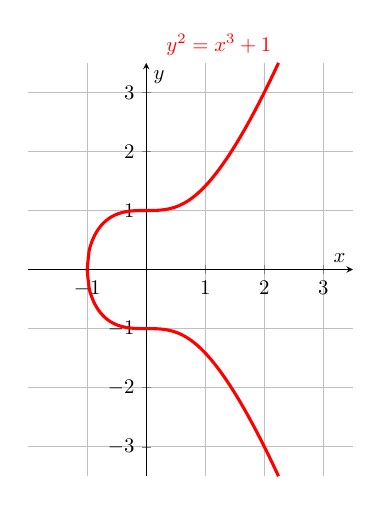
\begin{tikzpicture}[scale=0.75]
\newcommand{\avar}{0}
\newcommand{\bvar}{1}
\newcommand{\ymax}{3.5}
%\newcommand{\excx}{0.00008392}
\newcommand{\excx}{0}
\newcommand{\lw}{1.5}

\newcommand{\xmax}{2.24070237327858}
\newcommand{\xmin}{-1}
\begin{axis}
[grid=both,x=1cm,y=1cm,ymin=-3.5,ymax=3.5,xmax=3.5,xmin=-2,xtick={-1,...,3},ytick={-3,...,3},axis lines=middle,xlabel=$x$,ylabel=$y$,clip=false]
\draw [line width=\lw pt,smooth,samples=100,domain=\xmin-\excx:\xmax,color=red] plot(\x,{sqrt((\x)^3+\avar*\x+\bvar)});
\draw [line width=\lw pt,smooth,samples=100,domain=\xmin-\excx:\xmax,color=red] plot(\x,{-sqrt((\x)^3+\avar*\x+\bvar)});
\draw [above left,color=red] ({\xmax},\ymax) node {$y^2=x^3+1$};
\end{axis}
\end{tikzpicture}
}
\caption{Fibre at $t=0$.}
\end{subfigure}
\begin{subfigure}{0.3\textwidth}
\centering
\IfFileExists{../images/elliptic-fibres-zero.pdf}{\includegraphics{../images/elliptic-fibres-zero.pdf}}{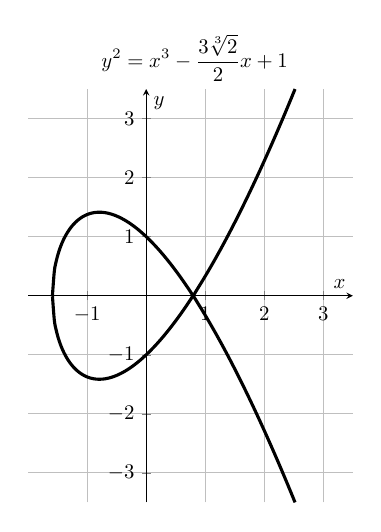
\begin{tikzpicture}[scale=0.75]
\newcommand{\avar}{-3/4^(1/3)}
\newcommand{\bvar}{1}
\newcommand{\ymax}{3.5}
%\newcommand{\exc}{0.006798}
\newcommand{\exc}{0.003579}
%\newcommand{\glum}{0.02}
\newcommand{\glum}{0.01}
%\newcommand{\glun}{0.15}
\newcommand{\glun}{0.2}
\newcommand{\lw}{1.5}

\newcommand{\xmax}{2.52055306100453}
\newcommand{\xmin}{-1.58740105196820}
\newcommand{\xnode}{0.793700525984100}
\begin{axis}
[grid=both,x=1cm,y=1cm,ymin=-3.5,ymax=3.5,xmax=3.5,xmin=-2,xtick={-1,...,3},ytick={-3,...,3},axis lines=middle,xlabel=$x$,ylabel=$y$,clip=false]
\draw [line width=\lw pt,smooth,samples=75,domain=\xmin:\xnode-\exc] plot(\x,{sqrt((\x)^3+\avar*\x+\bvar)});
\draw [line width=\lw pt,smooth,domain=\xnode+\exc:\xmax] plot(\x,{sqrt((\x)^3+\avar*\x+\bvar)});
\draw [line width=\lw pt,smooth,samples=75,domain=\xmin:\xnode-\exc] plot(\x,{-sqrt((\x)^3+\avar*\x+\bvar)});
\draw [line width=\lw pt,smooth,domain=\xnode+\exc:\xmax] plot(\x,{-sqrt((\x)^3+\avar*\x+\bvar)});
\draw [above left] ({\xmax},\ymax) node {$\displaystyle{y^2=x^3-\frac{3\sqrt[3]{2}}{2}x+1}$};
\draw [line width=\lw pt] ({\xmin},-\glum) -- ({\xmin},\glum);
\draw [fill] ({\xnode},0) circle (\glun pt);
\end{axis}
\end{tikzpicture}
}
\caption{Fibre at $t=-\frac{3\sqrt[3]{2}}{2}$.}
\end{subfigure}
\begin{subfigure}{0.3\textwidth}
\centering
\IfFileExists{../images/elliptic-fibres-pos.pdf}{\includegraphics{../images/elliptic-fibres-pos.pdf}}{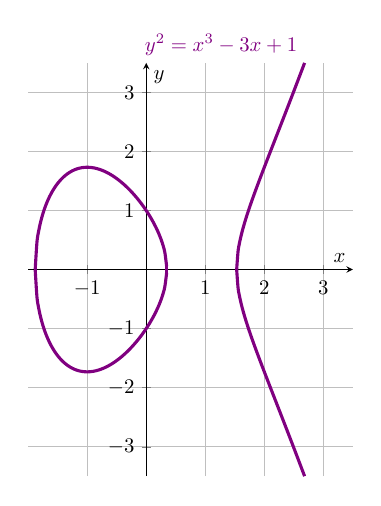
\begin{tikzpicture}[scale=0.75]
\newcommand{\avar}{-3}
\newcommand{\bvar}{1}
\newcommand{\ymax}{3.5}
%\newcommand{\exc}{0.000007630}
\newcommand{\exc}{0}
\newcommand{\glui}{0.009}
\newcommand{\gluii}{0.055}
\newcommand{\gluiii}{0.01}
\newcommand{\lw}{1.5}

\newcommand{\xmax}{2.68221750204240}
\newcommand{\xmin}{-1.87938524157182}
\newcommand{\xii}{0.347296355333861}
\newcommand{\xiii}{1.53208888623796}
\begin{axis}
[grid=both,x=1cm,y=1cm,ymin=-3.5,ymax=3.5,xmax=3.5,xmin=-2,xtick={-1,...,3},ytick={-3,...,3},axis lines=middle,xlabel=$x$,ylabel=$y$,clip=false]
\draw [line width=\lw pt,smooth,samples=75,domain=\xmin:\xii,color=violet] plot(\x,{sqrt((\x)^3+\avar*\x+\bvar)});
\draw [line width=\lw pt,smooth,samples=50,domain=\xiii+\exc:\xmax,color=violet] plot(\x,{sqrt((\x)^3+\avar*\x+\bvar)});
\draw [line width=\lw pt,smooth,samples=75,domain=\xmin:\xii,color=violet] plot(\x,{-sqrt((\x)^3+\avar*\x+\bvar)});
\draw [line width=\lw pt,smooth,samples=50,domain=\xiii+\exc:\xmax,color=violet] plot(\x,{-sqrt((\x)^3+\avar*\x+\bvar)});
\draw [above left,color=violet] ({\xmax},\ymax) node {$y^2=x^3-3x+1$};
\draw [line width=\lw pt,color=violet] ({\xmin},-\glui) -- ({\xmin},\glui);
\draw [line width=\lw pt,color=violet] ({\xii},-\gluii) -- ({\xii},\gluii);
\draw [line width=\lw pt,color=violet] ({\xiii},-\gluiii) -- ({\xiii},\gluiii);
\end{axis}
\end{tikzpicture}
}
\caption{Fibre at $t=-3$.}
\end{subfigure}
\caption{Representation in the real space of the elliptic surface $y^2=x^3+tx+1$ with its fibres at $t=0$ ($\Delta=-432$), $t=-\frac{3\sqrt[3]{2}}{2}$ ($\Delta=0$), $t=-3$ ($\Delta=1296$). The fibre at $t=a$ is obtained geometrically by intersecting the surface with the horizontal plane $t=a$.}
\label{fig:elliptic-surface}
\end{center}
\end{figure}

\subsection{Group law}

In Section \ref{Sse:elliptic-curves-group-law} we saw that an elliptic curve can be provided a group law. Silverman \cite[Section~III.3]{silverman1994advanced} extends this group law from elliptic curves to elliptic surfaces. Since almost all (all but finitely many) fibres of an elliptic surface are elliptic fibres, two points of the surface can be summed whenever they lie on the same elliptic fibre. This gives a rational map $X\times_CX\rightarrow X$ to the surface $X$, giving it a group scheme structure.

It is important to note that in $X\times_kX$ we wouldn't have an operation, because we cannot sum two points of different fibres. That's why we take the fibre product $X\times_CX$ over $C$, so that both points to be summed always belong to the same fibre.

It is also remarkable that not all fibres are elliptic fibres, so we can't define an operation on these non-singular fibres. However, the smooth fibres form an open dense subset of the surface, so the operation $X\times_CX\rightarrow X$ forms a rational map. There are also rational maps for the zero section $\sigma_0:C\rightarrow X$ and the inverse $X\rightarrow X$.

The sections of $\pi:X\rightarrow C$ are maps $\sigma:C\rightarrow X$ such that $\pi\circ\sigma=\id_C$. They can be viewed as selecting one point from each fibre -- respecting the algebraic and geometric structure. The zero elements in the fibres glue to a section called the \textbf{zero section} $\sigma_0$.

Sections are very worthy of study, because they let us ``extend'' the operation group also to singular fibres. Notice that, in general, a group scheme $X\rightarrow C$ with operation $\mu:X\times_CX\rightarrow C$ defines an operation on its set of sections
\begin{align*}
\mu:\Hom_{\Sch_C}(C,X)\times\Hom_{\Sch_C}(C,X)&\longrightarrow\Hom_{\Sch_C}(C,X),\\
(\sigma_1,\sigma_2)&\longmapsto\mu(\sigma_1,\sigma_2),
\end{align*}
defined through the following fibre product diagram:
\[
\begin{tikzcd}
&X\\
C\arrow[ru,"\sigma_1"]\arrow[rd,"\sigma_2"]\arrow[rr,"{(\sigma_1,\sigma_2)}"]&&X\times_CX\arrow[lu]\arrow[ld]\arrow[r,"\mu"]&X.\\
&X
\end{tikzcd}
\]

In our case, since $\mu$ is not a morphism, $\mu(\sigma_1,\sigma_2)$ is in principle not a section $C\rightarrow X$, but rather a rational map. However, since it is a rational map defined on a smooth curve, by \cite[Proposition~II.2.1]{silverman1986arithmetic}, it is a morphism, and hence, $\mu(\sigma_1,\sigma_2)\in\Hom_{\Sch_C}(C,X)$. This defines a group structure on the set of sections $\Hom_{\Sch_C}(C,X)$ of our elliptic surface $X\rightarrow C$.

We also have a group law on the points of the generic fibre $X_{\eta}$ that are rational over $k(C)$, since the generic fibre is an elliptic curve over the field $k(C)$. Silverman \cite[Proposition~3.10]{silverman1994advanced} shows that these group laws are compatible.

\begin{proposition}
Let $X\rightarrow C$ be an elliptic surface with generic fibre $X_{\eta}$ over a field $k$. There is a natural isomorphism of groups
\[\Hom_{\Sch_C}(C,X)\overset{\simeq}{\longrightarrow}\{P\in X_{\eta}\mid P\text{ rational over }k(C)\}.\]
\end{proposition}

\subsection{Hasse invariant}

\begin{definition}
Given an elliptic surface $X\rightarrow C$, we define its \textbf{Hasse invariant} as the Hasse invariant of its generic fibre $X_{\eta}\rightarrow\Spec k(C)$.
\end{definition}

As well as we can talk about supersingular elliptic curves, there is also a notion of supersingular elliptic surfaces. However, it involves the formal Brauer group and it is therefore explained in Chapter \ref{Cha:formal-brauer-group}.

\subsection{Singular fibres}

Given a general elliptic surface $X\rightarrow C$, most of the fibres are expected to be ordinary elliptic curves. Supersingular fibres are expected to be only a few of them. Even rarer is the case of singular fibres, which are the pathological cases, and there are only finitely many of them. However, most elliptic surfaces contain some singular fibres, so they must be taken into account.

Singular fibres of elliptic surfaces were first classified by Kodaira \cite[Theorem~6.2]{kodaira1963compact} for complex surfaces. Later, N\'{e}ron \cite[Section~III.17]{neron1964modeles} classified singular fibres in general characteristic. He showed that also for general fields, the singular fibres are those previously described by Kodaira (although N\'{e}ron gave them different names). Because of the importance of Kodaira's classification, his nomenclature is normally used in the literature.

A summarised classification of singular fibres is given by Sch\"{u}tt and Shioda \cite[Section~5.4]{schuett2019mordell} and is shown below.

\begin{theorem}
Let $X\rightarrow C$ be an elliptic surface with zero section $\sigma_0:C\rightarrow X$. Let $x\in C$ be a point where the fibre $X_x$ is singular. Let
\[X_x=\sum_{i=0}^{m-1}\mu_i\Theta_i\]
be its decomposition as a divisor into irreducible components, where for $0\leq i\leq m-1$, $\Theta_i$ is the $i$-th irreducible component, and has multiplicity $\mu_i$. The quantity $m$ is the number of different irreducible components.
Then, there exists a unique component that intersects the zero section $\sigma_0$. W.l.o.g. we say it is $\Theta_0$, and we call it the identity component. Its multiplicity is $\mu_0=1$.

The singular fibre $X_x$ either
\begin{enumerate}[label=(\roman*)]
\item is an irreducible singular fibre, i.e., $m=1$, $X_x=\Theta_0$ (types $\I_1$ and $\II$ detailed below); or
\item is a reducible singular fibre, i.e., $m>1$. In this case, all components $\Theta_i$ are smooth rational curves with self-intersection number $(\Theta_i)^2=-2$. (For more details about intersection numbers, see \cite[Lecture~12]{mumford1966lectures}.)
\end{enumerate}

The singular fibre $X_x$ is of one of the following types:

\begin{itemize}
\item[$\I_m$:]
\begin{itemize}
\item[$\I_1$:] $X_x=\Theta_0$ ($m=1$) is an irreducible rational curve with a node.
\item[$\I_2$:] $X_x=\Theta_0+\Theta_1$ ($m=2$) and the two components intersect transversally at two different points so that $(\Theta_0\cdot\Theta_1)=2$.
\item[$\I_m$:] $X_x=\Theta_0+\cdots+\Theta_{m-1}$ ($m\geq3$) where $(\Theta_i\cdot\Theta_{i+1})=1$ for all $i=0,\ldots,m-2$, and $(\Theta_{m-1}\cdot\Theta_0)=1$.
\end{itemize}

\item[$\II$:] $X_x=\Theta_0$ ($m=1$) is an irreducible rational curve with a cusp.

\item[$\III$:] $X_x=\Theta_0+\Theta_1$ ($m=2$) and both components intersect at one single point with $(\Theta_0\cdot\Theta_1)=2$.

\item[$\IV$:] $X_x=\Theta_0+\Theta_1+\Theta_2$ ($m=3$) and the three components meet at one single point with $(\Theta_0\cdot\Theta_1)=(\Theta_1\cdot\Theta_2)=(\Theta_2\cdot\Theta_0)=1$.

\item[$\I_b^*$:] $X_x=\Theta_0+\Theta_1+\Theta_2+\Theta_3+2\Theta_4+\cdots+2\Theta_{b+4}$ ($m=b+5$), $b\geq0$ with intersection numbers $(\Theta_0\cdot\Theta_4)=(\Theta_1\cdot\Theta_4)=(\Theta_2\cdot\Theta_{b+4})=(\Theta_3\cdot\Theta_{b+4})=1$, and $(\Theta_4\cdot\Theta_5)=\cdots=(\Theta_{b+3}\cdot\Theta_{b+4})=1$.

\item[$\II^*$:] $X_x=\Theta_0+2\Theta_7+3\Theta_6+4\Theta_5+5\Theta_4+6\Theta_3+4\Theta_2+2\Theta_1+3\Theta_8$ ($m=9$) with intersection numbers $(\Theta_0\cdot\Theta_7)=(\Theta_7\cdot\Theta_6)=(\Theta_6\cdot\Theta_5)=(\Theta_5\cdot\Theta_4)=(\Theta_4\cdot\Theta_3)=(\Theta_3\cdot\Theta_2)=(\Theta_2\cdot\Theta_1)=(\Theta_3\cdot\Theta_8)=1$.

\item[$\III^*$:] $X_x=\Theta_0+2\Theta_1+3\Theta_2+4\Theta_3+3\Theta_4+2\Theta_5+\Theta_6+2\Theta_7$ ($m=8$) with intersection numbers $(\Theta_0\cdot\Theta_1)=(\Theta_1\cdot\Theta_2)=(\Theta_2\cdot\Theta_3)=(\Theta_3\cdot\Theta_4)=(\Theta_4\cdot\Theta_5)=(\Theta_5\cdot\Theta_6)=(\Theta_3\cdot\Theta_7)=1$.

\item[$\IV^*$:] $X_x=\Theta_0+\Theta_1+2\Theta_2+3\Theta_3+2\Theta_4+\Theta_5+2\Theta_6$ ($m=7$) with intersection numbers $(\Theta_1\cdot\Theta_2)=(\Theta_2\cdot\Theta_3)=(\Theta_3\cdot\Theta_4)=(\Theta_4\cdot\Theta_5)=(\Theta_3\cdot\Theta_6)=(\Theta_6\cdot\Theta_0)=1$.
\end{itemize}

All pairs of irreducible components $\Theta_i\neq\Theta_j$ without an explicitly given intersection number are disjoint, i.e., $(\Theta_i\cdot\Theta_j)=0$.
\end{theorem}

\begin{figure}[!ht]
\begin{center}
\begin{subfigure}{0.45\textwidth}
\centering
\IfFileExists{../images/singular-fibres-1.pdf}{\includegraphics{../images/singular-fibres-1.pdf}}{\begin{tikzpicture}
\newcommand{\ymax}{1.5}
\newcommand{\xhead}{1.5}
\newcommand{\exc}{0.5}

\newcommand{\xmax}{(sqrt(((\ymax+\exc)/\xhead)^2*(27*((\ymax+\exc)/\xhead)^2-4))/(2*3^(3/2))+((\ymax+\exc)/\xhead)^2/2+(-1)/27)^(1/3)+1/(9*(sqrt(((\ymax+\exc)/\xhead)^2*(27*((\ymax+\exc)/\xhead)^2-4))/(2*3^(3/2))+((\ymax+\exc)/\xhead)^2/2+(-1)/27)^(1/3))+(-1)/3}
\draw [smooth,samples=75,domain=-1:0] plot(\xhead*\x,{\xhead*sqrt((\x)^(2)+(\x)^(3))});
\draw [smooth,domain=0:{\xmax}] plot(\xhead*\x,{\xhead*sqrt((\x)^(2)+(\x)^(3))});
\draw [smooth,samples=75,domain=-1:0] plot(\xhead*\x,{-\xhead*sqrt((\x)^(2)+(\x)^(3))});
\draw [smooth,domain=0:{\xmax}] plot(\xhead*\x,{-\xhead*sqrt((\x)^(2)+(\x)^(3))});
\end{tikzpicture}
}
\caption{Singular fibre of type $\I_1$.}
\end{subfigure}
\begin{subfigure}{0.45\textwidth}
\centering
\IfFileExists{../images/singular-fibres-2.pdf}{\includegraphics{../images/singular-fibres-2.pdf}}{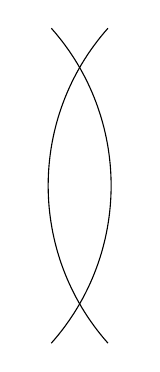
\begin{tikzpicture}
\newcommand{\ymax}{1.5}
\newcommand{\width}{0.4}
\newcommand{\exc}{0.5}

\draw ({(\ymax)^2/(2*\width)-\width/2-sqrt(((\ymax)^2/(2*\width)+\width/2)^2-(\ymax+\exc)^2)},\ymax+\exc) arc ({180-asin((\ymax+\exc)/((\ymax)^2/(2*\width)+\width/2))}:{180+asin((\ymax+\exc)/((\ymax)^2/(2*\width)+\width/2))}:{(\ymax)^2/(2*\width)+\width/2});
\draw ({-((\ymax)^2/(2*\width)-\width/2-sqrt(((\ymax)^2/(2*\width)+\width/2)^2-(\ymax+\exc)^2))},\ymax+\exc) arc ({asin((\ymax+\exc)/((\ymax)^2/(2*\width)+\width/2))}:{-asin((\ymax+\exc)/((\ymax)^2/(2*\width)+\width/2))}:{(\ymax)^2/(2*\width)+\width/2});
\end{tikzpicture}
}
\caption{Singular fibre of type $\I_2$.}
\end{subfigure}
\vspace{20mm}

\begin{subfigure}{0.45\textwidth}
\centering
\IfFileExists{../images/singular-fibres-3.pdf}{\includegraphics{../images/singular-fibres-3.pdf}}{\begin{tikzpicture}
\newcommand{\ymax}{1.5}
\newcommand{\exc}{0.5}

\draw ({-2*sqrt(3)/3*\ymax-sqrt(3)/3*\exc},{-\ymax-\exc}) -- ({sqrt(3)/3*\exc},{\ymax+\exc});
\draw ({-sqrt(3)/3*\exc},{\ymax+\exc}) -- ({2*sqrt(3)/3*\ymax+sqrt(3)/3*\exc},{-\ymax-\exc});
\draw ({2*sqrt(3)/3*\ymax+2*sqrt(3)/3*\exc},{-\ymax}) -- ({-2*sqrt(3)/3*\ymax-2*sqrt(3)/3*\exc},{-\ymax});
\end{tikzpicture}
}
\caption{Singular fibre of type $\I_3$.}
\end{subfigure}
\begin{subfigure}{0.45\textwidth}
\centering
\IfFileExists{../images/singular-fibres-4.pdf}{\includegraphics{../images/singular-fibres-4.pdf}}{\begin{tikzpicture}
\newcommand{\ymax}{1.5}
\newcommand{\exc}{0.5}

\draw ({-sqrt(3)/3*\ymax+sqrt(3)/3*\exc},{-\ymax-\exc}) -- ({-2*sqrt(3)/3*\ymax-sqrt(3)/3*\exc},\exc);
\draw ({-2*sqrt(3)/3*\ymax-sqrt(3)/3*\exc},-\exc) -- ({-sqrt(3)/3*\ymax+sqrt(3)/3*\exc},{\ymax+\exc});
\draw ({sqrt(3)/3*\ymax-sqrt(3)/3*\exc},{\ymax+\exc}) -- ({2*sqrt(3)/3*\ymax+sqrt(3)/3*\exc},-\exc);
\draw ({2*sqrt(3)/3*\ymax+sqrt(3)/3*\exc},\exc) -- ({sqrt(3)/3*\ymax-sqrt(3)/3*\exc},{-\ymax-\exc});
\draw (0,\ymax) node {$\cdots$};
\draw (0,-\ymax) node {$\cdots$};
\end{tikzpicture}
}
\caption{Singular fibre of type $\I_4$.}
\end{subfigure}
\caption{Illustration of the singular fibres of type $\I_m$ in an elliptic surface. Modified from: \cite[Figure~5.1]{schuett2019mordell}.}
\label{fig:singular-fibres}
\end{center}
\end{figure} 

Singular fibres are more difficult to study than non-singular fibres, as the latter are elliptic curves. For that reason, we would like to regularise singular fibres $X_s$ from an elliptic surface $X\rightarrow S$, if possible. One way is reduction. This process consists of doing a finite base change $S'\rightarrow S$ and take the new surface $X'=X\times_SS'\rightarrow S'$, and then potentially normalise. After this process, one may assume that all fibres are semi-stable, this is, smooth or singular of type $\I_m$, which is the ``least pathological'' case of singular fibres. A picture illustrating this type of singular fibres can be found in Figure \ref{fig:singular-fibres}.
%Try to find a source for this

\chapter{Formal groups}
\label{Cha:formal-groups}

In this chapter we will discuss about formal groups. First, we'll present formal group laws based on Liedtke's lectures on supersingular K3 surfaces \cite[Section~6.1]{liedtke2016lectures}. They are a very useful algebraic tool to describe formal group schemes. Of special interest is the \emph{height} of a formal group law, which is an invariant that allows to classify them. These formal groups appear as formal completions of group schemes, and they play an important role in the interplay between geometry and number theory.

\section{Formal group laws}

Let's start from the beginning: defining what a formal group law is. All rings considered in this work are commutative rings with unit.

\begin{definition}
\label{Def:formal_group}
Let $k$ be a ring. An $n$-dimensional \textbf{formal group law} $F$ is an $n$-tuple of formal power series $F=(F_1,\ldots,F_n)$ in $2n$ variables, say
\[F_i\in k\llbracket x_1,\ldots,x_n,y_1,\ldots,y_n\rrbracket,\]
denoting $x=(x_1,\ldots,x_n)$, $y=(y_1,\ldots,y_n)$, that satisfies two conditions:
\begin{enumerate}
\item\label{Def:formal_group:degree} $F_i(x,y)\equiv x_i+y_i$ mod $(x_1,\ldots,x_n,y_1,\ldots,y_n)^2$;
\item\label{Def:formal_group:associativity} $F_i(x,(F_i(y,z))=F_i(F_i(x,y),z)$.
\end{enumerate}

If $F$ further satisfies $F(x,y)=F(y,x)$, then $F$ is called \textbf{commutative}.
\end{definition}

Observe that $F$ can be seen as a formal group operation on $k^n$. When the components of $F$ are polynomials -- and thus have a finite amount of summands -- $F$ acts on $k^n$ as:
\begin{align*}
k^n\times k^n&\longrightarrow k^n.\\
(a,b)&\longrightarrow F(a,b)
\end{align*}
Condition \ref{Def:formal_group:degree} in Definition \ref{Def:formal_group} tells us that $F_i(x,y)=x_i+y_i$ plus some terms of degree greater than $1$. Hence, $F$ is the addition operation of $k$, plus some terms of higher order that are related with the infinitesimal behaviour of the group. Condition \ref{Def:formal_group:associativity} gives the associativity of the group.

Notice that we didn't require in the previous definition that there is an inverse. That's because, as Hazewinkel \cite[Section~II.9.1]{hazewinkel1978formal} states, the existence of an inverse is a consequence of the properties of the ring of formal power series.

\begin{remark}
Given an $n$-dimensional formal group law $F$, there exists a unique power series $\iota\in k\llbracket x_1,\ldots,x_n\rrbracket^n$ such that $F(x,\iota(x))=0$.
\end{remark}

We have two problems when we try to associate $F$ with the operation $k^n\times k^n\rightarrow k^n$:
\begin{enumerate}
\item $F$ carries more information than the operation on $k^n$. There may exist two formal group laws $F,G$ that are different as formal power series -- and thus are different -- but lead to the same operation $k^n\times k^n\rightarrow k^n$.
%Look for any concrete example

\item When $F$ has infinitely many terms, it cannot define an operation on $k^n$, as we would need a way to sum infinite terms. This can be solved either choosing a topology on the ring (like the $I$-adic topology) or taking only the nilpotent elements, as we can always apply a power series to them, because only finitely many terms are non-zero.
\end{enumerate}

Thus, we can associate the $n$-dimensional commutative formal group law $F$ over $k$ with a functor
\begin{align*}
\Phi_F:\Alg_k&\longrightarrow\Ab,\\
R&\longmapsto\sqrt{0}_{R^n},
\end{align*}
where $\Alg_k$ is the category of $k$-algebras and $\Ab$ is the category of abelian groups. We give the set $\sqrt{0}_{R^n}=\{(x_1,\ldots,x_n)\in R^n\,|\,x_1,\ldots,x_n\text{ are nilpotent}\}$ the group operation
\begin{align*}
\oplus_{\Phi_F}:\sqrt{0}_{R^n}\times\sqrt{0}_{R^n}&\longrightarrow\sqrt{0}_{R^n},\\
(a,b)&\longrightarrow F(a,b).
\end{align*}

This functor is an algebraic way of seeing formal group laws. But they can also be seen as the structure of completions of group schemes along the neutral element, as we will see in more detail in the following section.

\begin{definition}
A \textbf{homomorphism} $\alpha:F\rightarrow G$ between an $n$-dimensional formal group law $F$ and an $m$-dimensional formal group law $G$ is an $m$-tuple $\alpha=(\alpha_1,\ldots,\alpha_m)$ of formal power series in $n$ variables $x=(x_1,\ldots,x_n)$ such that:
\begin{enumerate}
\item $\alpha_i(x)\equiv0$ mod $(x_1,\ldots,x_n)$;
\item $\alpha(F(x,y))=G(\alpha(x),\alpha(y))$.
\end{enumerate}

A homomorphism $\alpha:F\rightarrow G$ is called an \textbf{isomorphism} when it has an inverse, i.e., when there exists a homomorphism $\beta:G\rightarrow F$ such that:
\begin{enumerate}
\item $\beta(\alpha(x))=x$,
\item $\alpha(\beta(y))=y$.
\end{enumerate}

An isomorphism is said to be \textbf{strict} when $\alpha_i(x)\equiv x_i$ mod $(x_1,\ldots,x_n)^2$.
\end{definition}

\begin{example}
Given an $m$-dimensional formal group law $F$, for an integer $n\geq1$, we can define the \textbf{multiplication by $\boldsymbol{n}$} as a formal power series $[n]\in k\llbracket x_1,\ldots,x_m\rrbracket^m$ defined by recurrence the following way:
\begin{itemize}
\item $[1](x)=x$,
\item $[n+1](x)=F([n](x),x)$, $n\geq1$.
\end{itemize}

It consists in applying $n$ times the operation of the group $F$. When $F$ is commutative, this defines a homomorphism $[n]:F\rightarrow F$.
%\vspace{3mm}

To get familiar with formal group laws, let's prove by induction step by step that $[n]$ is a homomorphism of formal group laws. For that, we need to prove that $[n](F(x,y))=F([n](x),[n](x))$.

For $n=1$, it is trivial. Assume it holds for some fixed $n\geq1$, and we'll prove it holds for $n+1$.

By induction hypothesis,
\[[n+1](F(x,y))=F([n](F(x,y)),F(x,y))=F\big(F([n](x),[n](y)),F(x,y)\big).\]
By associativity of $F$,
\[F\big(F([n](x),[n](y)),F(x,y)\big)=F\big(F\big(F([n](x),[n](y)),x\big),y\big).\]
By commutativity of $F$,
\[F\big(F\big(F([n](x),[n](y)),x\big),y\big)=F\big(F\big(x,F([n](x),[n](y))\big),y\big).\]
By associativity of $F$,
\[F\big(F\big(x,F([n](x),[n](y))\big),y\big)=F\big(F\big(F(x,[n](x)),[n](y)\big),y\big).\]
By commutativity of $F$,
\[F\big(F\big(F(x,[n](x)),[n](y)\big),y\big)=F\big(F\big(F([n](x),x)),[n](y)\big),y\big)=F\big(F([n+1](x),[n](y),y\big).\]
By associativity of $F$,
\[F\big(F([n+1](x),[n](y),y\big)=F\big([n+1](x),F([n](y),y)\big)=F([n+1](x),F([n+1](y)).\]
\hfill\qedsymbol

\end{example}

All formal group laws we will study will be commutative. In fact, Hazewinkel \cite[Section~I.6.1]{hazewinkel1978formal} proves that all $1$-dimensional formal group laws over a reduced ring are commutative.

\begin{example}
\label{exa:formal-additive-multiplicative}
The most simple examples of $1$-dimensional formal group laws are the following:
\begin{enumerate}
\item The \textbf{formal additive group}, denoted by $\widehat{\mathbb{G}}_a$, is defined by the formal power series $F(x,y)=x+y$.

\item The \textbf{formal multiplicative group}, denoted by $\widehat{\mathbb{G}}_m$, is defined by the formal power series $F(x,y)=x+y+xy$.
\end{enumerate}
\end{example}

Now, let's introduce an essential concept: the \emph{height}. It is an invariant that allows to classify formal group laws, and it is a central object of study in the formal groups that arise from algebraic varieties.

\begin{proposition}
Let $F$ be a $1$-dimensional commutative formal group law over a field $k$ of characteristic $p>0$. Consider the multiplication by $p$, $[p]:F\rightarrow F$. Then either $[p]=0$ or there exist an integer $s\geq1$ and $0\neq a\in k$ such that
\[[p](x)\equiv a\cdot x^{p^s}\text{ mod }(x^{p^s+1}).\]
\end{proposition}

\begin{definition}
Let $F$ be a $1$-dimensional commutative formal group law over a field $k$ of characteristic $p>0$. Consider the multiplication by $p$, $[p]:F\rightarrow F$. We define the \textbf{height} $h$ as follows:
\begin{itemize}
\item If $[p](x)=0$, then we define the height to be infinite, $h\coloneqq\infty$, and we call $F$ \textbf{unipotent}.

\item If $[p](x)\equiv ax^{p^s}$ mod $(x^{p^s+1})$, we define $h\coloneqq s$. In this case, we say that $F$ is \textbf{$\boldsymbol{p}$-divisible}.
\end{itemize}
\end{definition}

The importance of the height is due to the following theorem, that let's us uniquely characterise $1$-dimensional formal group laws.

\begin{theorem}
Let $k$ be an algebraically closed field of $\chara k=p>0$.
\begin{enumerate}
\item \cite[Corollaire~1]{lazard1955groupes} For every $h\geq1$ or $h=\infty$, there exists a $1$-dimensional abelian formal group law $F$ on $k$ with height $h$.
\item \cite[Th\'{e}or\`{e}me~IV]{lazard1955groupes} Two $1$-dimensional formal group laws on $k$ are isomorphic if and only if they have the same height.
\end{enumerate}
\end{theorem}

\section{Formal group schemes}

Formal group schemes -- also simply known as formal groups -- are the analogue of group schemes, but in the category of formal schemes. Thus, before talking about formal groups, let's define what formal schemes are.
%Talk about the infinitesimal idea behind completion and formal schemes

\subsection{Formal schemes}

The construction of formal schemes from topological rings is analogous to the construction of schemes from rings. First you define affine schemes, then you define general schemes as ringed spaces that are locally affine.

Let's start with topological rings. First, recall some definitions on $I$-adic rings given by Atiyah and MacDonald \cite[Chapter~10]{atiyah1969introduction}.

\begin{definition}
Given a ring $R$ and an ideal $I$, we can define the $I$-\textbf{adic topology} to be the topology in which every element $x\in R$ has $\{x+I^n\}_{n\in\mathbb{N}}$ as base of neighbourhoods.

We say that $R$ is an $I$-\textbf{adic ring} if it has the $I$-adic topology and it is separated (Hausdorff) and complete.
\end{definition}

For our geometric constructions, we will be interested in the completion of rings with respect to the $I$-adic topology. The completion thought of as the set of equivalent classes of Cauchy sequences might appear to be a highly abstract object, but here is a proposition that allows it to be calculated very easily.

\begin{proposition}
Given a ring $R$ with the $I$-adic topology, its completion can be written as an inverse limit:
\[\widehat{R}=\varprojlim R/I^n.\]
\end{proposition}

Grothendieck and Dieudonn\'{e} \cite[Section~I.10]{grothendieck1960elements} explain the theory of formal schemes that I present below.

\begin{definition}
%\cite[D\'{e}finition~I.10.1.2]{grothendieck1960elements}
%admissible anneaux = adic ring
Let $R$ be a noetherian $I$-adic ring. We define its \textbf{formal spectrum} as:
\[\Spf R=\Spec R/I.\]

On this topological space, we define the following structure sheaf:
\[\mathcal{O}_{\Spf R}=\varprojlim\mathcal{O}_{\Spec R/I^n}.\]
\end{definition}

\begin{remark}
The open prime ideals in $R$ are those that contain $I$. Hence, $\Spf R$ can be seen as the set of open prime ideals of $R$.
\end{remark}

The structure sheaf $\mathcal{O}_{\Spf R}$ of the formal spectrum is just the completion of the structure sheaf $\mathcal{O}_{\Spec R}$ of the spectrum. Hence, we have the following remark.

\begin{remark}
%\cite[Proposition~I.10.1.4]{grothendieck1960elements}
Given $f\in R$,
\[\mathcal{O}_{\Spf R}(D(f))=\widehat{R_f}.\]
\end{remark}

Notice that, even though $R$ is $I$-adically complete, we need to take the completion of the structure sheaf, because the localisations need not be complete.

\begin{definition}
%\cite[D\'{e}finition~I.10.4.2]{grothendieck1960elements}
Let $(X,\mathcal{O}_X)$ be a \textbf{topologically ringed space}, i.e., a sheaf of topological rings on the topological space $X$. We say that $(X,\mathcal{O}_X)$ is a \textbf{locally noetherian formal scheme} when every point $x\in X$ has an open neighbourhood $U\subseteq X$ isomorphic -- as topologically ringed spaces -- to the formal spectrum $(\Spf R,\mathcal{O}_{\Spf R})$ of some noetherian adic ring $R$.

We say that a locally noetherian formal scheme $(X,\mathcal{O}_X)$ is called \textbf{noetherian} if $X$ is quasi-compact. 
\end{definition}

Now we have the notion of a formal scheme. The following natural step is to define the morphisms between formal schemes. This is done the expected way.

\begin{definition}
%\cite[D\'{e}finition~I.10.4.5]{grothendieck1960elements}
Let $X,Y$ be formal schemes. A \textbf{morphism of formal schemes} $f:X\rightarrow Y$ is a morphism of the underlying ringed spaces with the extra condition of
\[f^{\sharp}(U):\mathcal{O}_Y(U)\longrightarrow\mathcal{O}_X(f^{-1}(U))\]
being continuous for every open set $U\subseteq Y$.
\end{definition}
%Extend definition of morphism of locally noetherian formal schemes to general formal schemes?

We have constructed formal schemes by means of completions of rings with respect to ideals. This can also be seen as the completion of an affine scheme (the spectrum of the ring) with respect to a closed subscheme (defined by the ideal). Grothendieck \cite[Section~2]{grothendieck1960geometrie} generalises the construction of formal schemes to completions of a generic scheme along a closed subscheme.

\begin{definition}
%\cite[D\'{e}finition~I.10.8.4]{grothendieck1960elements}
Let $X$ be a noetherian scheme and $Y$ a closed subscheme of $X$ with sheaf of ideals $\mathcal{I}$. Then we define the \textbf{completion of $\boldsymbol{X}$ along $\boldsymbol{Y}$} as the scheme $\widehat{X}=(Y,\mathcal{O}_{\widehat{X}})$ whose underlying topological space is $Y$ and whose sheaf of rings is the completion defined as
\[\mathcal{O}_{\widehat{X}}=\varprojlim\mathcal{O}_X/\mathcal{I}^n.\]
\end{definition}

\begin{example}
The most trivial example is the formal spectrum of a field $k$. In this case, if we complete $\Spec k$ along the $(0)$, we obtain $\Spf k$, that coincides with $\Spec k$, since the $0$-adic topology makes $k$ a discrete field, which is already complete.
\end{example}

Now that we know what formal schemes are, we are capable of defining formal groups.

\begin{definition}
A \textbf{formal group} is a group object in a category of formal schemes, usually the slice category of formal schemes over a field $k$ (more precisely, over $\Spf k$), or over some other formal scheme.
\end{definition}

\subsection{Formal group schemes as formal group laws}

So far, we have constructed formal schemes as completions of schemes, and we have defined formal groups, but we don't have any example yet on how to construct formal groups. Furthermore, formal group laws don't seem to be related with formal groups. In this section we will give a proceeding to construct formal groups, which will also reveal its interplay with formal group laws. A formal group law is a formal series, so it is easier to describe than a group scheme. Therefore, it will be very useful to represent a formal group as a formal group law. We will do that for formal groups arising from the completion of a group scheme along its neutral element. Liedtke presented this procedure in his lectures on supersingular K3 surfaces \cite[Example~6.10]{liedtke2016lectures}.

Let $G$ be a smooth commutative group scheme of dimension $n$ over a field $k$. Consider its neutral element $O\in G$. The local ring of $G$ at $O$ is $(\mathcal{O}_{G,O},\mathfrak{m})$. If we take its completion with respect to the $\mathfrak{m}$-adic topology, we get
\[\widehat{\mathcal{O}}_{G,O}=\varprojlim\mathcal{O}_{G,O}/\mathfrak{m}^m\cong k\llbracket x_1,\ldots,x_n\rrbracket=k\llbracket x\rrbracket,\]
with $x=(x_1,\ldots,x_n)$, since $G$ has dimension $n$ and it is non-singular at $O$. Then, $\widehat{G}=\Spf\widehat{\mathcal{O}}_{G,O}$ is the formal completion of $G$ along $O$.
%Check its compatibility with the previous definition

The multiplication $\mu:G\times_kG\rightarrow G$ extends to a multiplication operation on the formal scheme $\widehat{G}$, denoted as $\widehat{\mu}:\widehat{G}\times_k\widehat{G}\rightarrow\widehat{G}$. This multiplication is completely characterised by its corresponding $k$-algebra homomorphism
\[\widehat{\mu}^{\sharp}:k\llbracket x\rrbracket\longrightarrow k\llbracket y\rrbracket\widehat{\otimes}k\llbracket z\rrbracket\cong k\llbracket y,z\rrbracket,\]
where $\widehat{\otimes}$ refers to the completed tensor product. The image of $x$ determines uniquely the map $\widehat{\mu}^{\sharp}$. It can be checked that this formal power series $\widehat{\mu}^{\sharp}(x)\in k\llbracket y,z\rrbracket$ is indeed an $n$-dimensional formal group law. Thus, the operation of the formal group $\widehat{G}$ is uniquely determined by the formal group law $\widehat{\mu}^{\sharp}(x)\in k\llbracket y,z\rrbracket$.

\begin{example}
Completion along the origin justifies the definitions of the formal additive and multiplicative group laws in Example \ref{exa:formal-additive-multiplicative}. Indeed, the completion of the additive group scheme $\mathbb{G}_a$ along its origin is the formal additive group, which is represented by the formal additive group law $\widehat{\mathbb{G}}_a$. Likewise, the completion of the multiplicative group scheme $\mathbb{G}_m$ is represented by the formal multiplicative group law $\widehat{\mathbb{G}}_m$.
\end{example}

\begin{example}
Another example of this construction is the formal group of an elliptic curve. Recall the group scheme structure of an elliptic curve $X$ over a field $k$ as defined in Section \ref{Sse:elliptic-curves-group-law}. We can take the formal completion of $X$ along its neutral element $O$ to obtain its formal group $\widehat{X}$. Assume $\chara k>0$. From Theorem \ref{the:supersingular}, we know that the height $h$ of this formal group can tell us if $X$ is an ordinary ($h=1$) or a supersingular ($h=2$) elliptic curve.

Silverman \cite[Section~IV.1]{silverman1986arithmetic} provides an interesting description of the formal group of an elliptic curve in terms of the explicit power series. Let's present these calculations.

First take Weierstrass equation \eqref{eq:weierstrass-no-homo}:
\[y^2+a_1xy+a_3y=x^3+a_2x^2+a_4x+a_6,\]
expressed in inhomogeneous coordinates $x,y$. The neutral element $O$ is the infinity point $O=[0:1:0]$. Let's make it become the origin of inhomogeneous coordinates by doing the following change of coordinates:
\[t=-\frac{x}{y},\quad w=-\frac{1}{y}.\]
Then, Weierstrass equation turns into the following equation:
\begin{equation}
\label{Equ:neutral-origin}
w=t^3+a_1tw+a_2t^2w+a_3w^2+a_4tw^2+a_6w^3=f(t,w).
\end{equation}
Now, the neutral element has coordinates $(t,w)=(0,0)$. We want to study the differential behaviour of this elliptic curve around the origin. For that, we want to express the coordinate $w$ as a power series in $t$. We can achieve that by recursively substituting $w$ in Equation \eqref{Equ:neutral-origin} by its expression $f(t,w)$. This way, after the first step, we obtain:
\begin{align*}
w=t^3&+(a_1t+a_2t^2)\big(t^3+(a_1t+a_2t^2)w+a_3w^2+a_4tw^2+a_6w^3\big)\\
&+a_3\big(t^3+(a_1t+a_2t^2)w+a_3w^2+a_4tw^2+a_6w^3\big)^2\\
&+a_6\big(t^3+(a_1t+a_2t^2)w+a_3w^2+a_4tw^2+a_6w^3\big)^3.
\end{align*}
If we repeat the process indefinitely, we end up with an expression of the form
\[w(t)=t^3(1+A_1t+A_2t^2+\cdots),\]
for some coefficients $A_i\in\mathbb{Z}[a_1,\ldots,a_6]$ that are polynomials on the $a_j$. The first ones are:
\begin{align*}
A_1&=a_1,\\
A_2&=a_1^2+a_2,\\
A_3&=a_1^3+2a_1a_2+a_3,\\
A_4&=a_1^4+3a_1^2a_2+3a_1a_3+a_2^2+a_4.
\end{align*}

Since $w=f(t,w)$, this expression must satisfy $w(t)=f(t,w(t))$.

To define rigorously this process, we define by recurrence the polynomials
\[f_1(t,w)=f(t,w),\quad f_{m+1}(t,w)=f_m(t,f(t,w));\]
this is, each step we substitute the $w$ in $f_m$ by its equivalent expression $f(t,w)$. Silverman \cite[Proposition~IV.1.1]{silverman1986arithmetic} shows that this process converges.

\begin{proposition}
\begin{enumerate}[label=(\arabic*)]
\item The sequence of $f_m(t,0)$ in $\mathbb{Z}[a_1,\ldots,a_6]\llbracket t\rrbracket$ converges with the $(t)$-adic topology to a power series
\[w(t)=t^3(1+A_1t+A_2t^2+\cdots)\in\mathbb{Z}[a_1,\ldots,a_6]\llbracket t\rrbracket.\]
\item $w(t)$ is the unique power series in $\mathbb{Z}[a_1,\ldots,a_6]\llbracket t\rrbracket$ that satisfies $w(0)=0$ and $w(t)=f(t,f(w))$.
\end{enumerate}
\end{proposition}

This proposition is a consequence of Hensel's Lemma \cite[Lemma~IV.1.2]{silverman1986arithmetic}.

Now we can recover the original coordinates $x,y$ and express them as a Laurent series in $t$ with coefficients in $\mathbb{Z}[a_1,\ldots,a_6]$.
\[\frac{1}{w(t)}=\frac{1}{t^3}\,\frac{1}{1+A_1t+A_2t^2+\cdots}=\frac{1}{t^3}\big(1-(A_1t+A_2t^2+\cdots)+(A_1t+A_2t^2+\cdots)^2-\cdots\big),\]
\[x(t)=\frac{t}{w(t)}=\frac{1}{t^2}-\frac{a_1}{t}-a_2-a_3t-(a_4+a_1a_3)t^2-\cdots\]
\[y(t)=-\frac{1}{w(t)}=-\frac{1}{t^3}+\frac{a_1}{t^2}+\frac{a_2}{t}+a_3+(a_4+a_1a_3)t-\cdots\]
This expressions $(x(t),y(t))$ constitute a formal solution to Weierstrass equation \eqref{Equ:weierstrass}.

Now we can compute the sum of two points using the group law of the elliptic curve, and express it in terms of $t$. Take two variables $t_1,t_2$ that represent two points with their corresponding $w(t_1),w(t_2)$. The line in the plane $(w,t)$ that connects both points is given by $w=\lambda t+\nu$, where
\[\lambda=\lambda(t_1,t_2)=\frac{w_2-w_1}{t_2-t_1}=\sum_{n=3}^{\infty}A_{n-3}\frac{t_2^n-t_1^n}{t_2-t_1}\in\mathbb{Z}[a_1,\ldots,a_6]\llbracket t_1,t_2\rrbracket,\]
\[\nu=\nu(t_1,t_2)=w_1(t_1)-\lambda(t_1,t_2)t_1\in\mathbb{Z}[a_1,\ldots,a_6]\llbracket t_1,t_2\rrbracket.\]
Now, this line intersects the elliptic curve in a third point $t_3$ given by
\[t_3=t_3(t_1,t_2)=-t_1-t_2-\frac{a_1\lambda+a_3\lambda^2+a_2\nu+2a_4\lambda\nu+3a_6\lambda^2\nu}{1+a_2\lambda+a_4\lambda^2+a_6\lambda^3}\in\mathbb{Z}[a_1,\ldots,a_6]\llbracket t_1,t_2\rrbracket,\]
and $w_3$ can be given equivalently by $w_3=w(t_3(t_1,t_2))$ or by
\[w_3=\lambda(t_1,t_2)t_3(t_1,t_2)+\nu(t_1,t_2).\]
So far, we got the three collinear points $(t_1,w_1)$, $(t_2,w_2)$, $(t_3,w_3)$, meaning that $(t_3,w_3)$ is the inverse of the sum $(t_1,w_1)+(t_2,w_2)$, so we just need to invert it. In usual coordinates $(x,y)$ the inverse is given by $(x,-y-a_1x-a_3)$, so it can be expressed as a power series in $t$ as:
\[\iota(t)=\frac{x(t)}{y(t)+a_1x(t)+a_3}=\frac{t^{-2}-a_1t^{-1}-\cdots}{-t^{-3}+2a_1t^{-2}+\cdots}\in\mathbb{Z}[a_1,\ldots,a_6]\llbracket t\rrbracket.\]
Hence, the formal group law of the elliptic curve results in:
\begin{align*}
F(t_1,t_2)&=\iota(t_3(t_1,t_2))\\
&=t_1+t_2-a_1t_1t_2-a_2(t_1^2t_2+t_1t_2^2)+(-2a_3t_1^3t_2+(a_1a_2-3a_3)t_1^2t_2^2-2a_3t_1t_2^3)+\cdots\in\mathbb{Z}[a_1,\ldots,a_6]\llbracket t_1,t_2\rrbracket.
\end{align*}

With this, we have given an explicit calculation of the formal group law that represents the formal group arising as the completion of the group law of an elliptic surface along its neutral element.
\end{example}

%\section{Formal group functors}
%https://encyclopediaofmath.org/wiki/Formal_group

\chapter{\'{E}tale cohomology}

Cohomology on schemes arises from the fact that, given a scheme $X$, the functor taking global sections of $\mathcal{O}_X$-modules
\[\Gamma(X,-):\mathfrak{Mod}_{\mathcal{O}_X}\longrightarrow\Mod_{\Gamma(X,\mathcal{O}_X)}\]
is left exact, but it not right exact. So for each $\mathcal{O}_X$-module $\mathcal{F}$, we can define its cohomology $H^{\bullet}(X,\mathcal{F})$.

For example, for complex varieties $X$, cohomology on the Euclidean topology is very used. One can, for instance, define the Betti numbers $b_r(X)$ as the dimensions of the cohomology groups $H^r(X(\mathbb{C}),\mathbb{Q})$, regarded as vector spaces over $\mathbb{C}$. However, for a general variety over a generic field, we only have the Zariski topology, which is too coarse. For example, if $X$ is irreducible, then the groups $H^r(X,\mathbb{Z})$ are zero for all $r>0$ for the Zariski topology. To solve this, Grothendieck proposed a finer topology that allowed to develop a useful cohomology theory. This is the \'{e}tale topology -- although it is not a topology strictly speaking, but a more general notion called \emph{site}.

With this new tool, we can do cohomology of finite groups $\Lambda$ over general fields. For the particular case of complex varieties, the \'{e}tale cohomology groups $H^r(X_{\text{\'{e}t}},\Lambda)$ coincide with the cohomology groups $H^r(X(\mathbb{C}),\Lambda)$ for the usual Euclidean topology

In this chapter we will expose the theory of \'{e}tale topology, mainly based on Milne's lectures \cite{milne2013lectures}. This will be later used in Chapter \ref{Cha:formal-brauer-group} to define the formal Brauer group.

\section{Sites}

If we define a sheaf of abelian groups, and then we want to define a sheaf of rings, formally we should give again the definition for these presheaves, although the procedure is completely analogous. Therefore, one may want to define sheaves of objects of a general category. (For a detailed explanation about category theory, see \cite{maclane1971categories}.)

Usually, a presheaf $\mathcal{F}$ is defined as a family of abelian groups $\mathcal{F}(U)$ (or sets, rings\ldots) indexed on the open sets $U$ of a topological space $X$, together with restriction maps $\rho_{UV}:\mathcal{F}(U)\rightarrow\mathcal{F}(V)$ whenever $V\subseteq U\subseteq X$, and such that $\rho_{UW}=\rho_{VW}\circ\rho_{UV}$ whenever $W\subseteq V\subseteq U$.

Observe that this can be rewritten in the language of categories. Consider the category $\Top(X)$ defined as follows:
\begin{itemize}
\item The objects of $\Top(X)$ are the open sets of the topology of $X$.

\item Given $U,V\subseteq X$ open sets, there exists a morphism and only one $V\rightarrow U$ if and only if $V\subseteq U$. This can be interpreted as the morphisms being the inclusions.

\item The composition of morphisms is the only one possible: given $W\rightarrow V$ and $V\rightarrow U$, the composition is the only morphism $W\rightarrow U$.
\end{itemize}

With this, observe that a presheaf of objects in a category $C$ can be defined as just a contravariant functor
\[\mathcal{F}:\Top(X)\rightarrow C.\]
The inclusion $V\hookrightarrow U$ is mapped by the functor $\mathcal{F}$ into the restriction $\rho_{UV}:\mathcal{F}(U)\rightarrow\mathcal{F}(V)$.
\vspace{2mm}

The notion of sheaf can be translated into the language of categories too. A presheaf $\mathcal{F}$ is called a sheaf when it satisfies the axioms of separatedness and glueing, this is, when for all open set $U\subseteq X$ and open cover $\{U_i\}_{i\in I}$ of $U$, if we have $\{s_i\in\mathcal{F}(U_i)\}_{i\in I}$ such that $\forall i,j\in I$ $\rho_{U_i,U_i\cap U_j}(s_i)=\rho_{U_j,U_i\cap U_j}(s_j)$, then there exists a unique $s\in\mathcal{F}(U)$ such that $\forall i\in I$ $\rho_{UU_i}(s)=s_i$.

This definition works well when we have a concrete category. But in a more general category, we need a more general definition. Assume that the category $C$ has all limits. Let $U\subseteq X$ be open with open cover $\{U_i\}_{i\in I}$. Consider the following maps:
%Only small limits are needed?
\[(\rho_{UU_i})_{i\in I}:\mathcal{F}(U)\longrightarrow\prod_{i\in I}\mathcal{F}(U_i),\]
this is, the morphism whose $i$-th component is $\rho_{UU_i}$.
Let
\[\pi_i:\prod_{i\in I}\mathcal{F}(U_i)\longrightarrow\mathcal{F}(U_i)\]
be the projection onto the $i$-th component. Then, consider
\[(\rho_{U_i,U_i\cap U_j}\circ\pi_i)_{i,j\in I}:\prod_{i\in I}\mathcal{F}(U_i)\longrightarrow\prod_{i,j\in I}\mathcal{F}(U_i\cap U_j);\]
\[(\rho_{U_j,U_i\cap U_j}\circ\pi_j)_{i,j\in I}:\prod_{i\in I}\mathcal{F}(U_i)\longrightarrow\prod_{i,j\in I}\mathcal{F}(U_i\cap U_j).\]

Then the condition of $\mathcal{F}$ being a sheaf is equivalent to $\mathcal{F}(U)$, together with the map $(\rho_{UU_i})_{i\in I}$, being the equaliser of $(\rho_{U_i,U_i\cap U_j}\circ\pi_i)_{i,j\in I}$ and $(\rho_{U_j,U_i\cap U_j}\circ\pi_j)_{i,j\in I}$ for all $U\in\Top(X)$. This is the following equaliser diagram:
\begin{equation}
\label{Equ:sheaf_equaliser}
\begin{tikzcd}
\mathcal{F}(U)\arrow[r]&\displaystyle{\prod_{i\in I}\mathcal{F}(U_i)}\arrow[r,shift left]\arrow[r,shift right]&\displaystyle{\prod_{i,j\in I}\mathcal{F}(U_i\cap U_j)}.
\end{tikzcd}
\end{equation}

Also observe that the fact that $C$ has limits implies the existence of a terminal object $t$. Taking $U=\emptyset$ and the empty covering $\{U_i\}_{i\in\emptyset}$, the empty product is the terminal object, so the sheaf condition writes as:
\[
\begin{tikzcd}
\mathcal{F}(\emptyset)\arrow[r]&t\arrow[r,shift left]\arrow[r,shift right]&t,
\end{tikzcd}
\]
so $\mathcal{F}(\emptyset)$ is the terminal object in $C$, because $t$ is the equaliser of $t\rightrightarrows t$.
\vspace{2mm}

Once defined what a sheaf is, we need to define the morphisms of sheaves. Morphisms $\varphi:\mathcal{F}\rightarrow\mathcal{G}$ between presheaves are usually defined as families of morphisms indexed on $\Top(X)$ such that:
\begin{enumerate}
\item $\forall U\subseteq X$ open, $\varphi(U):\mathcal{F}(U)\rightarrow\mathcal{G}(U)$ is a morphism in $C$;
\item $\forall V\subseteq U\subseteq X$ open, the following diagram commutes:
\[
\begin{tikzcd}
\mathcal{F}(U)\arrow[r,"\varphi(U)"]\arrow[d,"\rho_{UV}^{\mathcal{F}}"]&\mathcal{G}(U)\arrow[d,"\rho_{UV}^{\mathcal{G}}"]\\
\mathcal{F}(V)\arrow[r,"\varphi(V)"]&\mathcal{G}(V).
\end{tikzcd}
\]
\end{enumerate}

This is nothing, but a natural transformation $\varphi:\mathcal{F}\Rightarrow\mathcal{G}$ from the contravariant functor $\mathcal{F}$ to the contravariant functor $\mathcal{G}$. Morphisms of sheaves are just defined as morphisms of presheaves between sheaves. All this argumentation leads to the following definition.

\begin{definition}
Let $X$ be a topological space and let $C$ be a category with all limits. The \textbf{category of presheaves} is defined as the functor category
\[\PSh_X(C)=C^{\Top(X)^{\text{op}}}.\]
The \textbf{category of sheaves} $\Sh_X(C)$ is the full subcategory of $\PSh_X(C)$ whose objects satisfy the sheaf condition \eqref{Equ:sheaf_equaliser}.
\end{definition}
\vspace{2mm}

Now, we have defined what a sheaf from a topology to a general category with all limits is. This notion is still limited, because it is restricted to be defined on categories that can be expressed as a topology. Therefore, we would like to extend the notion of sheaf to more general categories.

The notion of presheaf can be directly extended to a general category, since it doesn't use any special characteristics of a topology. However, the definition of a sheaf involves open covers, which a general category doesn't have. Thus, Milne \cite[Section~I.5]{milne2013lectures} extends the notion of covering.

\begin{definition}
\label{Def:site}
A \textbf{site} is a category $C$ together with what is called a \textbf{coverage}. A coverage, also referred to as \textbf{(Grothendieck) topology}, associates for each object $U$ in $C$ the set of all its coverings. Coverings of $U$ are families of morphisms $\{U_i\rightarrow U\}_{i\in I}$ that satisfy the following axioms:
\begin{enumerate}
\item\label{Def:site:coverage_product} For any covering $\{U_i\rightarrow U\}_{i\in I}$ and any morphism $V\rightarrow U$ in $C$, the fibre products $U_i\times_UV$ exist and $\{U_i\times_UV\rightarrow V\}_{i\in I}$ is a covering of $V$.

\item If $\{U_i\rightarrow U\}_{i\in I}$ is a covering of $U$, and for each $i\in I$, $\{V_{ij}\rightarrow U_i\}_{j\in J_i}$ is a covering of $U_i$, then $\{V_{ij}\rightarrow U\}_{i\in I,j\in J_i}$ is a covering of $U$.

\item For any $U$ in $C$, $\{\id:U\rightarrow U\}$ consisting of a single map is a covering.
\end{enumerate}
\end{definition}

We have defined what a site is. Let's now define the notion of morphism between sites. Since they are seen as generalisations of topologies, these morphisms are called continuous maps.

\begin{definition}
%\cite[Definition~I.5.2]{milne2013lectures}
Let $\boldsymbol{T}_1,\boldsymbol{T}_2$ be sites. A \textbf{continuous map} $\boldsymbol{T}_1\rightarrow\boldsymbol{T}_2$ between sites is a functor on the underlying categories $\Cat(\boldsymbol{T}_2)\rightarrow\Cat(\boldsymbol{T}_1)$ that preserves fibre products and coverings.
\end{definition}

\begin{remark}
A topological space $X$, with its category of open sets $\Top(X)$ and its usual coverings is a site. It is denoted $X_{\text{zar}}$, as it is the Zariski topology regarded as a site.

In $X_{\text{zar}}$, given an open set $U$ and an open cover $\{U_i\}_{i\in I}$, the family of inclusions $\{U_i\rightarrow U\}_{i\in I}$ form the associated covering.

Notice that the fibre product in this case is just the intersection, since for open sets $U_1,U_2\subseteq V$, it satisfies the following universal diagram:
\[
\begin{tikzcd}
W\arrow[rrd,bend left]\arrow[rdd,bend right]\arrow[rd,dashed]\\
&U_1\cap U_2\arrow[r]\arrow[d]&U_2\arrow[d]\\
&U_1\arrow[r]&V.
\end{tikzcd}
\]

This way, condition \ref{Def:site:coverage_product} in Definition \ref{Def:site} reads as: any covering of $U$, if intersected with $V$, gives a covering of $V$, which we know is true.
\vspace{2mm}

Continuous maps between topological spaces $f:X\rightarrow Y$ give rise to continuous maps of their associated sites via the functor $f^{-1}:\Top(Y)\rightarrow\Top(X)$.
\end{remark}

\begin{definition}
Given a site $\boldsymbol{T}$, we define a \textbf{presheaf} of objects in a category $C$ to be a contravariant functor $\mathcal{F}:\boldsymbol{T}\rightarrow C$.

A presheaf is called a \textbf{sheaf} if it satisfies the \textbf{sheaf axiom}:
\[
\begin{tikzcd}
\mathcal{F}(U)\arrow[r]&\displaystyle{\prod_{i\in I}\mathcal{F}(U_i)}\arrow[r,shift left]\arrow[r,shift right]&\displaystyle{\prod_{i,j\in I}\mathcal{F}(U_i\times_UU_j)}
\end{tikzcd}
\]
is the equaliser diagram for all coverings $\{U_i\rightarrow U\}_{i\in I}$ of $U$.

\textbf{Morphisms of presheaves and sheaves} are, as before, the natural transformations.
\end{definition}

\begin{remark}
When the site is a topology, we recover the usual definition of sheaf, since the fibre product is the intersection.
\end{remark}

\section{\'{E}tale morphisms}

To subsequently define the \'{e}tale topology, Milne \cite[Section~I.2]{milne2013lectures} introduces a new property of morphisms of schemes: \'{e}tale morphisms. For that, let's first recall some definitions of various properties of morphisms of schemes.

\begin{definition}
A homomorphism of rings $f:A\rightarrow B$ is called \textbf{flat} if it realises $B$ as a flat $A$-module, i.e., if the functor $\otimes_AB:\Mod_A\rightarrow\Mod_A$ is exact.
\end{definition}

\begin{definition}
A morphism of schemes $f:X\rightarrow Y$ is called \textbf{flat} if $\forall x\in X$ the local homomorphisms of rings $f_x^{\sharp}:\mathcal{O}_{Y,f(x)}\rightarrow\mathcal{O}_{X,x}$ are flat.

It is sufficient to check the flatness on closed points.
\end{definition}

\begin{definition}
A homomorphism of local rings $f:A\rightarrow B$ is called \textbf{unramified} if:
\begin{enumerate}
\item $f(\mathfrak{m}_A)B=\mathfrak{m}_B$, and
\item $B/\mathfrak{m}_B$ is a finite separable field extension of $A/\mathfrak{m}_A$.
\end{enumerate}
\end{definition}

\begin{definition}
A morphism of schemes $f:X\rightarrow Y$ is called \textbf{unramified} if it is unramified at all points, i.e., if $\forall x\in X$ $f_x^{\sharp}:\mathcal{O}_{Y,f(x)}\rightarrow\mathcal{O}_{X,x}$ is unramified.

It is sufficient to check the unramified property on closed points.
\end{definition}

Now that we have defined flat and unramified morphisms, let's introduce the notion of \'{e}tale morphisms.

\begin{definition}
A morphism of schemes $f:X\rightarrow Y$ is called \textbf{\'{e}tale} if it is flat and unramified.
\end{definition}

This definition may appear to be merely algebraic, so here is a result on varieties that helps understand the geometric meaning of \'{e}tale morphisms. Recall that a variety $X$ over an algebraically closed field $k$ is a separated integral scheme of finite type over $k$.

\begin{proposition}
%\cite[Proposition~I.2.9]{milne2013lectures}
Let $f:X\rightarrow Y$ be a smooth morphism of smooth varieties over an algebraically closed field $k$. Then $f$ is \'{e}tale if and only if $\forall x\in X$ the map on tangent spaces
%In the book it says "nonsingular" instead of "smooth". Be careful
\[df_x:(\mathfrak{m}_x/\mathfrak{m}_x^2)^{\vee}\longrightarrow\big(\mathfrak{m}_{f(x)}/\mathfrak{m}_{f(x)}^2\big)^{\vee}\]
is an isomorphism.
\end{proposition}

This proposition tells us that \'{e}tale morphisms are maps whose differential is an isomorphism of tangent spaces at every point. Recall that in differential geometry, by the inverse map theorem, this type of functions are local diffeomorphisms. Hence, \'{e}tale morphisms are the algebraic analogue to local diffeomorphisms.

Let's see some basic properties of \'{e}tale morphisms.

\begin{proposition}
\label{Pro:etale_properties}
%\cite[Proposition~I.2.11]{milne2013lectures}
\begin{enumerate}
\item\label{Pro:etale_properties:immersion} All open immersions are \'{e}tale.

\item The composition of two \'{e}tale morphisms is again \'{e}tale.

\item Every base change of an \'{e}tale morphism is \'{e}tale.

\item\label{Pro:etale_properties:component} If $\varphi\circ\psi$ and $\varphi$ are both \'{e}tale, then $\psi$ is \'{e}tale as well.
\end{enumerate}
\end{proposition}

\section{\'{E}tale cohomology}

\subsection{\'{E}tale topology}

Now that we have the notions of \'{e}tale morphisms and sites, let's construct the \'{e}tale site, mostly known as ``\'{e}tale topology'' (although it is not a topology in the usual sense), on which we will define sheaves, schemes and eventually cohomology.

\begin{definition}
%\cite[Section~I.1]{milne2013lectures}
Let $X$ be a scheme. We define the \textbf{\'{e}tale site} $X_{\text{\'{e}t}}$ -- or \textbf{\'{e}tale topology} -- as follows:
\begin{enumerate}
\item The underlying category, called $\Et(X)$, is the slice category where objects are schemes $U$ together with \'{e}tale morphisms $U\rightarrow X$. Morphisms between from an object $U\rightarrow X$ to another object $V\rightarrow X$ are the \'{e}tale morphisms $U\rightarrow V$ that make the following diagram commute:
\[
\begin{tikzcd}[column sep=small]
U\arrow[rr]\arrow[rd]&&V\arrow[ld]\\
&X.
\end{tikzcd}
\]

\item The coverings of $U\rightarrow X$ are the families $\{\varphi_i:U_i\rightarrow U\}_{i\in I}$ of morphisms in $\Et(X)$ such that
\[U=\bigcup_{i\in I}\varphi_i(U_i).\]
\end{enumerate}
\end{definition}
In the \'{e}tale topology, \'{e}tale morphisms $U\rightarrow X$ act as the ``open sets'' of the topology, in analogy to the usual notion of topology.

\begin{remark}
\begin{enumerate}
\item The same scheme $U$ can give rise to different objects in $\Et(X)$ when taken two different \'{e}tale morphisms $U\rightrightarrows X$.

\item Every open subset $U\subseteq X$ has a unique structure of open subscheme $U\hookrightarrow X$. Thanks to Proposition \ref{Pro:etale_properties}.\ref{Pro:etale_properties:immersion}, the immersion $U\hookrightarrow X$ is \'{e}tale. Hence, $\Top(X)$ is a subcategory of $\Et(X)$. Furthermore, all coverings in $X_{\text{zar}}$ are also coverings in $X_{\text{\'{e}t}}$. Therefore, the \'{e}tale topology is finer than the Zariski topology, i.e., all open subsets of $X$ are also open in the \'{e}tale topology. This also gives a continuous map $X_{\text{\'{e}t}}\rightarrow X_{\text{zar}}$. (Note that the continuous map reverses order with respect to the functor of underlying categories.)

\item Let $U\rightarrow X$, $U_i\rightarrow X$ for $i\in I$ be elements of $\Et(X)$ -- i.e., \'{e}tale morphisms -- and let $\{U_i\rightarrow U\}_{i\in I}$ be an arbitrary family of morphisms of schemes that cover $U$ and commute:
\[
\begin{tikzcd}
U_i\arrow[r]\arrow[rd]&U\arrow[d]\\
&X.
\end{tikzcd}
\]
This family automatically constitutes a covering of $U$ in $X_{\text{\'{e}t}}$, since $U_i\rightarrow U$ are \'{e}tale by Proposition \ref{Pro:etale_properties}.\ref{Pro:etale_properties:component}.
\end{enumerate}
\end{remark}

\subsection{Sheaves on the \'{e}tale topology}

So far, we have defined what sheaves on the \'{e}tale topology are. They are not just objects that exist, but Milne \cite[Section~I.6]{milne2013lectures} also constructs explicit examples of such sheaves. Let's do the most typical ones.

\subsubsection*{Coherent $\boldsymbol{\mathcal{O}_X}$-module}

Let $\mathcal{F}$ be a coherent sheaf of modules on a scheme $X$. Let $\varphi:U\rightarrow X$ be an \'{e}tale morphism. Then, the inverse image $\varphi^*\mathcal{F}$ is a coherent sheaf on $U$. Take
\[\mathcal{F}^{\text{\'{e}t}}(U)\coloneqq H^0(U,\varphi^*\mathcal{F}|_U).\]
It can be checked that this leads to a sheaf $\mathcal{F}^{\text{\'{e}t}}$ on $X_{\text{\'{e}t}}$, where the restriction maps are given as follows: to a morphism $\rho:U\rightarrow V$ of \'{e}tale opens corresponds the inverse image map
\[\rho^*:\mathcal{F}^{\text{\'{e}t}}(V)\longrightarrow\mathcal{F}^{\text{\'{e}t}}(U).\]

In particular, we can take the structure sheaf $\mathcal{F}=\mathcal{O}_X$ of the scheme $X$. Following the previous construction, we can obtain the structure sheaf $\mathcal{O}_{X_{\text{\'{e}t}}}$ on the site $X_{\text{\'{e}t}}$.

\subsubsection*{Stalks}

\begin{definition}
%\cite[Section~I.4.Schemes]{milne2013lectures}
Let $X$ be a scheme over an algebraically closed $k$. A \textbf{geometric point} of $X$ is a morphism of schemes $\bar{x}:\Spec k\rightarrow X$.

An \textbf{\'{e}tale neighbourhood} of $\bar{x}$ is a pair of an \'{e}tale morphism $U\rightarrow X$ and a geometric point $\bar{u}:\Spec k\rightarrow U$ such that the following diagram commutes:
\[
\begin{tikzcd}[row sep=small]
&U\arrow[dd]\\
\Spec k\arrow[ru,"\bar{u}"]\arrow[rd,swap,"\bar{x}"]\\
&X.
\end{tikzcd}
\]

%\cite[Section~I.6.Stalks]{milne2013lectures}
Let $\mathcal{F}$ be a presheaf on $X_{\text{\'{e}t}}$. The \textbf{stalk} of $\mathcal{F}$ at the geometric point $\bar{x}$ defined as:
\[\mathcal{F}_{\bar{x}}\coloneqq\varinjlim_{(U,\bar{u})}\mathcal{F}(U),\]
where the direct limit is taken over all \'{e}tale neighbourhoods $(U,\bar{u})$ of $\bar{x}$.
\end{definition}

\begin{example}
\begin{enumerate}
%\cite[Section~I.4.The case of varieties]{milne2013lectures}
\item In the case of the structure sheaf $\mathcal{O}_{X_{\text{\'{e}t}}}$, the stalk at $\bar{x}:\Spec k\rightarrow X$ takes the form
\[\mathcal{O}_{X,\bar{x}}=\varinjlim_{(U,\bar{u})}H^0(U,\mathcal{O}_U),\]
where the direct limit is taken over all connected affine \'{e}tale neighbourhoods $(U,\bar{u})$ of $\bar{x}$. The ring $\mathcal{O}_{X,\bar{x}}$ is often referred to as the \textbf{strictly local ring} at $\bar{x}$.

Every open subset $U\subseteq X$ that contains $x$ is an \'{e}tale neighbourhood of $\bar{x}$ via the inclusion $U\hookrightarrow X$ and the geometric point $\bar{u}$ that factorises $\bar{x}$:
\[
\begin{tikzcd}[column sep=small]
\Spec k\arrow[rr,"\bar{x}"]\arrow[rd,swap,"\bar{u}"]&&X.\\
&U\arrow[ru,hook]
\end{tikzcd}
\]
Hence, there are morphisms $H^0(U,\mathcal{O}_U)\rightarrow\mathcal{O}_{X,\bar{x}}$ (compatible with restrictions) for all open sets $U\subseteq X$. By the universal property of the direct limit, there exists a unique ring homomorphism $\mathcal{O}_{X,x}\rightarrow\mathcal{O}_{X,\bar{x}}$ such that the following diagram commutes:
\[
\begin{tikzcd}[column sep=small,row sep=small]
&\mathcal{O}_{X,\bar{x}}\\\\
&\mathcal{O}_{X,x}\arrow[uu,dashed]\\
H^0(U,\mathcal{O}_U)\arrow[rr]\arrow[ru]\arrow[ruuu,bend left]&&H^0(V,\mathcal{O}_V).\arrow[lu]\arrow[luuu,bend right]
\end{tikzcd}
\]

%\cite[Example~I.6.13]{milne2013lectures}
\item More generally, the stalk of a coherent $\mathcal{O}_X$-module $\mathcal{F}$ at $\bar{x}$ is
\[\mathcal{F}_x\otimes_{\mathcal{O}_{X,x}}\mathcal{O}_{X,\bar{x}},\]
where $\mathcal{F}_x$ is the usual stalk of $\mathcal{F}$ as a sheaf on $X_{\text{zar}}$, and $x\in X$ is the image of the point in $\Spec k$ by the map $\bar{x}$.
\end{enumerate}
\end{example}

\subsubsection*{Skyscraper sheaf}

Now, we would like to define the skyscraper sheaf on the \'{e}tale topology. Recall that in the case of a topological space $X$, a skyscraper sheaf $\mathcal{F}$ is such that for some $x\in X$, $\mathcal{F}_x=\Lambda$ for some abelian group $\Lambda$, while for all $y\neq x$, $\mathcal{F}_x=0$. This can be constructed as the sheafification of the presheaf
\[\mathcal{F}(U)=\left\{\begin{array}{rcl}\Lambda&\text{if}&x\in U,\\0&\text{if}&x\notin U;\end{array}\right.\]
which results in the direct sum of $\Lambda$ indexed on all the connected components of $U$.

\begin{definition}
%\cite[Section~I.6.Skyscraper sheaves]{milne2013lectures}
Let $X$ be a variety over an algebraically closed field $k$, $x\in X$, and let $\Lambda$ be an abelian group. We define the \textbf{skyscraper sheaf} $\Lambda^x$ on $X_{\text{\'{e}t}}$ as follows: for any \'{e}tale map $\varphi:U\rightarrow X$, write
\[\Lambda^x(U)\coloneqq\bigoplus_{u\in\varphi^{-1}(x)}\Lambda.\]
\end{definition}

It can be checked that $\Lambda^x$ is indeed a sheaf on $X_{\text{\'{e}t}}$, and it is such that for $y\notin\varphi(U)$, $\Lambda^x(U)=0$.

\begin{remark}
Taking the stalk at $x$ is the left adjoint functor of taking the skyscraper sheaf of the abelian group. This means, there exists a natural bijection
\[\Hom(\mathcal{F},\Lambda^x)\simeq\Hom(\mathcal{F},\Lambda).\]
This tells us that to give a morphism of sheaves $\mathcal{F}\rightarrow\Lambda^x$, it is sufficient to give a morphism of abelian groups $\mathcal{F}\rightarrow\Lambda$.
\end{remark}

\subsubsection*{Constant sheaf}

Another very useful construction using abelian groups is the constant sheaf.
%\cite[Section~I.6.Examples of sheaves on $X_{\text{et}}$]{milne2013lectures}

\begin{definition}
Let $X$ be a quasi-compact scheme and let $\Lambda$ be an abelian group. For $U\rightarrow X$ \'{e}tale, define
\[\mathcal{F}_{\Lambda}(U)=\Lambda^{\pi_0(U)},\]
this is, a family of copies of $\Lambda$ indexed $\pi_0(U)$, the set of connected components of $U$. $\mathcal{F}_{\Lambda}$ defines a sheaf of abelian groups on $X_{\text{\'{e}t}}$, called the \textbf{constant sheaf} defined by $\Lambda$. Many times, the sheaf $\mathcal{F}_{\Lambda}$ is simply denoted as $\Lambda$.
\end{definition}

\begin{remark}
If $\Lambda$ is a finite group, then its constant sheaf is defined by $X\times\Lambda$ -- disjoint union of copies of $X$ indexed on $\Lambda$.
\end{remark}

These sheaves are used very often in \'{e}tale cohomology. As said at the beginning of this chapter, \'{e}tale topology was firstly developed with the goal of doing cohomology of groups on varieties. That's why constructing sheaves out of abelian groups is so relevant. In the following section, we will see an example of these cohomology groups.

%
An important tool that Milne \cite[Section~I.8]{milne2013lectures} defines is the inverse image of a sheaf.

\begin{definition}
%\cite[Section~I.8.Inverse images of sheaves]{milne2013lectures}
Let $f:X\rightarrow Y$ be a morphism of schemes. Let $\mathcal{F}$ be a sheaf on $Y_{\text{\'{e}t}}$. We define the presheaf $\mathcal{F}'$ on $X_{\text{\'{e}t}}$ as:
\[\mathcal{F}'(V)=\varinjlim\mathcal{F}(U),\]
for $V\rightarrow X$ \'{e}tale, and the direct limit is taken over \'{e}tale morphisms $U\rightarrow Y$ such that the following diagram commutes:
\[
\begin{tikzcd}
V\arrow[r]\arrow[d]&U\arrow[d]\\
X\arrow[r]&Y.
\end{tikzcd}
\]
We define the \textbf{inverse image} $f^*\mathcal{F}$ to be the sheafification of $\mathcal{F}'$.
\end{definition}

\begin{proposition}
%\cite[Remark~I.8.9]{milne2013lectures}
Given a morphism of schemes $f:X\rightarrow Y$, the inverse image $f^*\Sh(Y_{\text{\'{e}t}})\rightarrow\Sh(X_{\text{\'{e}t}})$ is an exact functor.
\end{proposition}


\subsection{\'{E}tale cohomology}

We have defined the category of sheaves on $X_{\text{\'{e}t}}$, so know we are prepared to do cohomology on it. As Milne \cite[Section~I.7]{milne2013lectures} explains, taking global sections is not a right-exact functor (same as in the case of Zariski topologies), so we will perform cohomology on its right-derived functor. In this section, $X$ will always be a variety.

\begin{proposition}
%\cite[Proposition~I.7.6]{milne2013lectures}
Let $\mathcal{F}',\mathcal{F},\mathcal{F}''$ be sheaves on $X_{\text{\'{e}t}}$. Then
\[0\longrightarrow\mathcal{F}'\longrightarrow\mathcal{F}\longrightarrow\mathcal{F}''\longrightarrow0\]
is exact if and only if for all geometric point $\bar{x}\rightarrow X$, the following short sequence is exact:
\[0\longrightarrow\mathcal{F}'_{\bar{x}}\longrightarrow\mathcal{F}_{\bar{x}}\longrightarrow\mathcal{F}''_{\bar{x}}\longrightarrow0.\]

%\cite[Proposition~I.7.5]{milne2013lectures}
However, we can only say that
\[0\longrightarrow\mathcal{F}'\longrightarrow\mathcal{F}\longrightarrow\mathcal{F}''\]
is exact if and only if for all \'{e}tale morphisms $U\rightarrow X$, the following sequence is exact:
\[0\longrightarrow\mathcal{F}'(U)\longrightarrow\mathcal{F}(U)\longrightarrow\mathcal{F}''(U).\]
\end{proposition}

This proposition tells us exactly that the functor
\begin{align*}
\Gamma(U,-):\Sh_{X_{\text{\'{e}t}}}(\Ab)&\longrightarrow\Ab\\
\mathcal{F}&\longmapsto\mathcal{F}(U)
\end{align*}
is left exact. But it is not right exact.

The following proposition provided by Milne \cite[Proposition~I.8.12]{milne2013lectures} gives us the injectives we need to construct the cohomology.

\begin{proposition}
%\cite[Proposition~I.8.12]{milne2013lectures}
The category $\Sh_{X_{\text{\'{e}t}}}(\Ab)$ of sheaves of abelian groups on $X_{\text{\'{e}t}}$ has enough injectives. This means, for every sheaf $\mathcal{F}$ there exists an injective sheaf $\mathcal{I}$ and an injective morphism of sheaves $\mathcal{F}\rightarrow\mathcal{I}$.
\end{proposition}

%\cite[Section~I.9]{milne2013lectures}
Now, we have all the tools to construct the \'{e}tale cohomology \cite[Section~I.9]{milne2013lectures}. The existence of enough injectives allows the construction of injective resolutions
\[\mathcal{F}\longrightarrow\mathcal{I}_0\longrightarrow\mathcal{I}_1\longrightarrow\mathcal{I}_2\longrightarrow\cdots\]
to which apply the functor $\Gamma(U,-)$ to obtain the complex
\[\mathcal{F}(U)\longrightarrow\mathcal{I}_0(U)\overset{d_0}{\longrightarrow}\mathcal{I}_1(U)\overset{d_1}{\longrightarrow}\mathcal{I}_2(U)\longrightarrow\cdots\]
which is not exact and has cohomology groups
\[H^i(U,\mathcal{F})=\frac{\ker d_i}{\im d_{i-1}}.\]
%Are these sections in U or in X?

\begin{remark}
The cohomology groups do not depend on the injective resolution. Hence, we can apply the general theory of derived functors. It states that for all $r\geq0$, we have a well defined functor:
\begin{align*}
H^r(X_{\text{\'{e}t}},-):\Sh_{X_{\text{\'{e}t}}}(\Ab)&\longrightarrow\Ab\\
\mathcal{F}&\longrightarrow H^r(X_{\text{\'{e}t}},\mathcal{F})
\end{align*}
that is the $r$-th right derived functor of $\Gamma(X,-)$. It satisfies the following properties:
\begin{enumerate}
\item for any sheaf $\mathcal{F}$, $H^0(X_{\text{\'{e}t}},\mathcal{F})=\mathcal{F}(X)$;
\item for an injective sheaf $\mathcal{I}$, $H^r(X_{\text{\'{e}t}},\mathcal{I})=0$ $\forall r\geq1$;
\item for a short exact sequence of sheaves
\[0\longrightarrow\mathcal{F}'\longrightarrow\mathcal{F}\longrightarrow\mathcal{F}''\longrightarrow0,\]
we have a long exact sequence
\[
\begin{tikzcd}
0\arrow[r]&\underbrace{H^0(X_{\text{\'{e}t}},\mathcal{F}')}_{\mathcal{F}'(X)}\arrow[r]&\underbrace{H^0(X_{\text{\'{e}t}},\mathcal{F})}_{\mathcal{F}(X)}\arrow[r]&\underbrace{H^0(X_{\text{\'{e}t}},\mathcal{F}'')}_{\mathcal{F}''(X)}\arrow[lld,out=345,in=165,looseness=1.4]\\
&H^1(X_{\text{\'{e}t}},\mathcal{F}')\arrow[r]&H^1(X_{\text{\'{e}t}},\mathcal{F})\arrow[r]&H^1(X_{\text{\'{e}t}},\mathcal{F}'')\arrow[lld,out=350,in=170,looseness=1.4]\\
&H^2(X_{\text{\'{e}t}},\mathcal{F}')\arrow[r]&H^2(X_{\text{\'{e}t}},\mathcal{F})\arrow[r]&H^2(X_{\text{\'{e}t}},\mathcal{F}'')\arrow[lld,out=355,in=175,looseness=1.4,shorten >= -2.5cm]\\
&\null&\ldots
\end{tikzcd}
\]
\end{enumerate}
\end{remark}

\subsubsection*{$\boldsymbol{\ell}$-adic cohomology}

Liedtke \cite[Section~1.3]{liedtke2016lectures} provides an example of usage of \'{e}tale cohomology: the Betti numbers, which are cohomological invariants of varieties that arise from the $\ell$-adic cohomology.

\begin{definition}
Let $X$ be a smooth variety over a field of characteristic $p\geq0$. Let $\ell$ be a prime number. We define the $n$-th $\ell$-\textbf{adic cohomology} group of $X$ to be
\[H_{\text{\'{e}t}}^n(X,\mathbb{Z}_{\ell})\coloneqq\varprojlim H_{\text{\'{e}t}}^n(X,\mathbb{Z}/\ell^m\mathbb{Z}),\]
where $\mathbb{Z}/\ell^m\mathbb{Z}$ is regarded as the constant sheaf on $X_{\text{\'{e}t}}$.

Define as well
\[H_{\text{\'{e}t}}^n(X,\mathbb{Q}_{\ell})\coloneqq H_{\text{\'{e}t}}^n(X,\mathbb{Z}_{\ell})\otimes_{\mathbb{Z}_{\ell}}\mathbb{Q}_{\ell}.\]
\end{definition}

Observe that we didn't define the cohomology groups to be directly $H_{\text{\'{e}t}}^n(X,\mathbb{Q}_{\ell})$. That's because it's preferred to do \'{e}tale cohomology on finite abelian groups. Hence, we perform cohomology on $\mathbb{Z}/\ell^m\mathbb{Z}$, and after that, extend it to the ring $\mathbb{Z}_{\ell}$ of $\ell$-adic integers, and then to the field $\mathbb{Q}_{\ell}$ of $\ell$-adic numbers.

Something about cohomology groups we are often interested in is their dimension. Let's present a result proven by Katz and Messing \cite[Corollary~1]{katz1974consequences} on the dimension of the $\ell$-adic cohomology groups.

\begin{proposition}
Let $X$ be a smooth proper variety over an algebraically closed field $k$ of positive characteristic $p>0$. Let $\ell\neq p$ be a prime number. Then, the dimension of $H_{\text{\'{e}t}}^n(X,\mathbb{Q}_{\ell})$ over $\mathbb{Q}_{\ell}$ does not depend on $\ell$.
\end{proposition}

This result let's us define a very useful invariant of these varieties.

\begin{definition}
\label{def:betti-numbers}
Let $X$ be a smooth proper variety over an algebraically closed field $k$ of positive characteristic $p>0$. We define the $n$-th \textbf{Betti number} of $X$ as
\[b_n(X)=\dim_{\mathbb{Q}_{\ell}}H_{\text{\'{e}t}}^n(X,\mathbb{Q}_{\ell}),\]
for some prime $\ell\neq p$.
\end{definition}

In Chapter \ref{Cha:formal-brauer-group}, we will show the close relation of the Betti numbers with the formal Brauer group, and they will help to calculate some of its properties, such as its height.

\chapter{Formal Brauer group}
\label{Cha:formal-brauer-group}

Artin and Mazur \cite{artin1977formal} presented a family of formal group laws that arise from algebraic varieties. I will expose here what Liedtke \cite[Section~6.2]{liedtke2016lectures} presented about these formal group laws.

Given a variety $X$ over an algebraically closed field $k$, we can define for every algebra $k\rightarrow R$, the fibre product $X\times_{\Spec k}\Spec R$, which we will call, for the sake of simplicity, $X\times_kR$.

\begin{definition}
Let $X$ be a smooth proper variety over a field $k$. For each $n\geq1$, we define the following functor:
\begin{align*}
\Phi_X^n:\Art_k&\longrightarrow\Ab,\\
R&\longmapsto\ker\left(H_{\text{\'{e}t}}^n(X\times_kR,\mathcal{O}_{X\times_kR}^{\times})\xrightarrow{\text{res}}H_{\text{\'{e}t}}^n(X,\mathcal{O}_X^{\times})\right),
\end{align*}
where $\Art_k$ is the category of local Artinian $k$-algebras with residue field $k$, $\Ab$ is the category of abelian groups, $\mathcal{O}_X^{\times}$ is the sheaf of invertible elements of $\mathcal{O}_X$.
%What map is "res"?
\end{definition}

This functor is especially interesting when it is prorepresentable by a formal group, as it can be given a geometric structure. The prorepresentability is discussed in \cite{artin1977formal}, and it is known in some special cases.
%Present the definition of prorepresentability

\begin{example}
The case $n=1$ is very well known, and is explained by Liedtke \cite[Example~6.14]{liedtke2016lectures}. The elements in the cohomology group $H_{\text{\'{e}t}}^1(X\times_kR,\mathcal{O}_{X\times_kR}^{\times})$ can be identified with the invertible sheaves over $X\times_kR$. Hence, $\Phi_X^1(R)$ is identified with the group of invertible sheaves on $X\times_kR$ that are trivial when restricted to $X$. Thus, there is a bijection
\[\Phi_R^1(X)\longleftrightarrow\{f:\Spec R\rightarrow\Pic_{X/k}\,|\,f\text{ maps }\mathfrak{m}_R\text{ to the class of }\mathcal{O}_X\},\]
where $\Pic_{X/k}$ is the Picard scheme of $X$. (For more information about the construction of the Picard scheme, see \cite{kleiman2005picard}.) Thus, there is a natural isomorphism of functors
\[\Phi_X^1\cong\widehat{\Pic}_{X/k},\]
where $\widehat{\Pic}_{X/k}$ is the formal completion of the Picard scheme $\Pic_{X/k}$ along its neutral element. Hence, $\Phi_X^1$ is prorepresentable by a commutative formal group law if and only if $\Pic_{X/k}^0$ -- which is the connected component of $\Pic_{X/k}$ that contains the zero -- is smooth over $k$, i.e., when $\Pic_{X/k}^0$ is an abelian variety. In this case, we call it the \textbf{formal Picard group}. It has dimension $\dim_kH^1(X,\mathcal{O}_X)$.
\end{example}

Ideally, one could expect an analogous case for $n=2$: if there were a ``Brauer scheme'', its tangent space should be $H^2(X,\mathcal{O}_X)$, and the functor $\Phi_X^2$ should be prorepresentable by the formal completion of this Brauer scheme along the zero. However, this is not the case. Nonetheless, under certain conditions, $\Phi_X^2$ is prorepresentable, so it still can be studied in this direction.

\begin{definition}
We define the \textbf{(cohomological) Brauer group} of the scheme $X$ as the cohomology group
\[H_{\text{\'{e}t}}^2(X,\mathcal{O}_X^{\times}).\]
\end{definition}

Then, $\Phi_X^2$ studies the deformations of the neutral element of the Brauer group $H_{\text{\'{e}t}}^2(X,\mathcal{O}_X^{\times})$. Let's study it for a special type of surfaces, the so-called K3 surfaces, also explained by Liedtke \cite[Section~2]{liedtke2016lectures}.

\begin{definition}
%\cite[Definition~2.1]{liedtke2016lectures}
A surface $X$ is called a \textbf{K3 surface} when it is a smooth and projective surface over a field $k$ and it is such that $\omega_X\cong\mathcal{O}_X$ and $h^1(X,\mathcal{O}_X)=0$.
\end{definition}

The usefulness of K3 surfaces comes from the following proposition.

\begin{proposition}
Let $X$ be a smooth proper variety over a field $k$. Assume that $h^1(X,\mathcal{O}_X)=h^3(X,\mathcal{O}_X)$ (this is the case, for instance, of K3 surfaces). Then, the functor $\Phi_X^2$ is prorepresentable by a commutative formal group law. This formal group law has dimension equal to $h^2(X,\mathcal{O}_X)$.
\end{proposition}

\begin{definition}
In the assumptions of the previous proposition, the formal group law that prorepresents $\Phi_X^2$ is called the \textbf{formal Brauer group} of $X$, and is denoted as $\widehat{\Br}_X\coloneqq\Phi_X^2$.
\end{definition}

So in some cases, $\Phi_X^2$ is known to be prorepresentable. For $n\geq3$, however, much less is known about the functor $\Phi_X^n$. So, we will study the formal Brauer group ($n=2$) for K3 surfaces.

\section{K3 surfaces}

An important remark about K3 surfaces is the following.

\begin{remark}
In a K3 surface, the geometric and the arithmetic genus coincide. Therefore, we will simply refer to its genus $g$.
\end{remark}
%The genus of all K3 surfaces is 1

\begin{proof}
On the one hand, the geometric genus is, by definition:
\[p_g(X)=h^0(X,\omega_X).\]
On the other hand, the arithmetic genus is defined in terms of the Euler characteristic, which in dimension $2$ is:
\[p_a(X)=(-1)^2\big(\chi(\mathcal{O}_X)-1\big)=h^2(X,\mathcal{O}_X)-h^1(X,\mathcal{O}_X).\]
By definition of K3 surface, the ``irregularity'' $h^1(X,\mathcal{O}_X)=0$ vanishes. Furthermore, by Serre duality, $h^2(X,\mathcal{O}_X)=h^0(X,\omega_X)$. Thus,
\[p_a(X)=h^2(X,\mathcal{O}_X)-h^1(X,\mathcal{O}_X)=h^0(X,\omega_X)-0=p_g(X)=g(X).\]
\end{proof}

Also, K3 surfaces have specific cohomological invariants, which allow to do further computations. Let's first present its Betti numbers \cite[Proposition~2.3]{liedtke2016lectures}.

\begin{proposition}
\label{pro:k3-betti}
Let $X$ be a K3 surface. Then, $X$ has the following Betti numbers:
\begin{align*}
b_0(X)&=1,\\
b_1(X)&=0,\\
b_2(X)&=22,\\
b_3(X)&=0,\\
b_4(X)&=1.
\end{align*}
\end{proposition}

One can also compute the Hodge numbers $h^{pq}(X)\coloneqq\dim_kH^q(X,\bigwedge^p\Omega_X)$ \cite[Proposition~2.4]{liedtke2016lectures}. They are usually given in the form of a Hodge diamond.

\begin{proposition}
A K3 surface has the following Hodge diamond:
\[\begin{tikzcd}[column sep=-3pt,row sep=3pt]&&h^{00}\\&h^{10}&&h^{01}\\h^{20}&&h^{11}&&h^{02}\\&h^{21}&&h^{12}\\&&h^{22}\end{tikzcd}\qquad=\qquad\begin{tikzcd}[column sep=1pt,row sep=3pt]&&1\\&0&&0\\1&&20&&1\\&0&&0\\&&1\end{tikzcd}\]
\end{proposition}

Let's give a method \cite[Example~2.2]{liedtke2016lectures} to construct explicit examples of K3 surfaces using coordinates inside the projective space.

\begin{proposition}
Let $k$ be an algebraically closed field. Let $X$ be a smooth quartic surface in $\mathbb{P}_k^3$, i.e., a smooth closed subscheme of $\mathbb{P}_k^3$ of degree $4$ and of dimension $2$. Then $X$ is a K3 surface.
\end{proposition}

\begin{proof}
Two things are to be shown:
\begin{enumerate}
\item $\omega_X\cong\mathcal{O}_{\mathbb{P}_k^3}$. Let $\mathcal{I}$ be the sheaf of ideals associated to $X$. Since we are in codimension $1$, the adjunction formula takes the following form:
\[\omega_X\cong\omega_{\mathbb{P}_k^3}\otimes\mathcal{I}^{\vee}\otimes\mathcal{O}_X.\]
Now, since $X$ has degree $4$, $\mathcal{I}=\mathcal{O}_{\mathbb{P}_k^3}(-4)$. Furthermore, $\omega_{\mathbb{P}_k^3}=\mathcal{O}(-4)$. Thus,
\[\omega_X\cong\mathcal{O}(-4)\otimes\mathcal{O}(4)\otimes\mathcal{O}_X=\mathcal{O}_X.\]
%Check on which sheaf of rings the tensor product is performed

\item $H^1(X,\mathcal{O}_X)=0$. Recall that from Hartshorne \cite[Theorem~III.5.1]{hartshorne1977algebraic} that $H^i(\mathbb{P}_k^d,\mathcal{O}_{\mathbb{P}_k^d}(n))=0$ for all $n\in\mathbb{Z}$ and all $i\notin\{0,d\}$. If $i:X\hookrightarrow\mathbb{P}_k^3$ is the inclusion, the closed subscheme exact sequence writes:
\[0\longrightarrow\mathcal{I}\longrightarrow\mathcal{O}_{\mathbb{P}_k^3}\longrightarrow i^*\mathcal{O}_X\longrightarrow0.\]
Taking cohomology, we get
\[H^1(\mathbb{P}_k^3,\mathcal{O}_{\mathbb{P}_k^3})\longrightarrow H^1(\mathbb{P}_k^3,i^*\mathcal{O}_X)\longrightarrow H^2(\mathbb{P}_k^3,\mathcal{I}).\]
Now, since $\mathcal{I}$ is a sheaf of ideals and, in particular, an invertible sheaf, $H^2(\mathbb{P}_k^3,\mathcal{I})$. Furthermore, $H^1(\mathbb{P}_k^3,\mathcal{O}_{\mathbb{P}_k^3})=0$. Thus,
\[H^1(\mathbb{P}_k^3,i^*\mathcal{O}_X)=0.\]
Finally, by the compatibility of cohomology with inverse images,
\[H^1(X,\mathcal{O}_X)=H^1(\mathbb{P}_k^3,i^*\mathcal{O}_X)=0.\]
\end{enumerate}
\end{proof}
%Give Fermat's quartic as an example of non-vacuous study

So now we can restrict ourselves to the study of the properties of the formal Brauer group for the special case of a degree $4$ surface in the projective space, as they will automatically be K3, so they will have an associated formal Brauer group. We will assume further that the surface $X$ is given a map $X\rightarrow C$ onto a curve $C$ that makes it an elliptic surface.

Let's first recall the N\'{e}ron--Severi group of a scheme. For that, let's take the definition for algebraic equivalence of divisors that Hartshorne \cite[Exercise~V.7]{hartshorne1977algebraic} provides.

\begin{definition}
\label{def:neron-severi-group}
Let $X$ be a surface (i.e., a nonsingular projective variety of dimension $2$ over an algebraically closed field $k$). Let $T$ be a nonsingular curve over $k$. $X\times T$ is a family of fibres $X_t$ isomorphic to $X$ indexed by $T$. Let $D$ be an effective Cartier divisor on $X\times T$ that is flat as a closed scheme of $X\times T$. Then, for each closed point $t\in T$ in the curve, the intersection $D_t=D.X_t$ between $D$ and the fibre $X_t$ defines a Cartier divisor $D_t$ on $X_t\cong X$. Then, we say that $\{D_t\,|\,t\in T\}$ is an \textbf{algebraic family of divisors} on $X$ parametrised by $T$.

For all closed points $t_0,t_1\in T$, we say that the divisors $D_{t_0},D_{t_1}$ are prealgebraically equivalent. Two general divisors $D,D'\in\Div(X)$ are said to be prealgebraically equivalent if they are differences of prealgebraically equivalent effective divisors. Finally, we say that two divisors $D,D'\in\Div(X)$ are \textbf{algebraically equivalent} if there exists a finite sequence $D=D_0,D_1,\ldots,D_{n-1},D_n=D'$ such that $D_i$ and $D_{i+1}$ are prealgebraically equivalent for $i=0,\ldots,n-1$.

The group of divisors of a surface $X$ modulo algebraic equivalence is called the \textbf{N\'{e}ron--Severi group}, and is denoted $\NS(X)$.
\end{definition}

\begin{remark}
\begin{enumerate}
\item The divisors algebraically equivalent to $0$ form a subgroup of $\Div(X)$. This fact tells us that the N\'{e}ron--Severi group is indeed a group.

\item Linearly equivalent divisors are also algebraically equivalent. This makes the principal divisors a subgroup of the divisors algebraically equivalent to $0$.
\end{enumerate}
\end{remark}

Lang and N\'{e}ron \cite{lang1959rational} proved the following theorem using the theorem of the base.

\begin{theorem}[Lang--Neron]
The N\'{e}ron--Severi group $\NS(X)$ of a surface $X$ is finitely generated.
\end{theorem}

Recall (for example, from \cite[Chapter~I]{lang1965algebra}, Sections \emph{Direct sums and free abelian groups} and \emph{Finitely generated abelian groups}) that a finitely generated abelian group $G$ has an associated rank $n$, which is the nonnegative integer such that $G/G_{\text{tor}}\cong\mathbb{Z}^n$, where $G_{\text{tor}}=\{x\in G\,|\,\exists n>0:nx=0\}$ is the torsion group of $G$. This leads to the following definition \cite{moonen1993picard}.
%\cite[I,~Theorem~4]{lang1965algebra} and \cite[I,~Theorem~8]{lang1965algebra} in first edition
%\cite[I,~Theorem~7.3]{lang1965algebra} and \cite[I,~Theorem~8.5]{lang1965algebra} in third edition

\begin{definition}
The previous theorem allows us to define the \textbf{rank of the N\'{e}ron--Severi group} of a surface, which is often denoted as $\rho$. This quantity is also called the \textbf{Picard number} of the surface.
\end{definition}

But in the case of elliptic surfaces, Sch\"{u}tt and Shioda \cite[Theorem~6.2]{schuett2009elliptic} state that we don't need to care about the torsion of the N\'{e}ron--Severi group because of the following theorem.

\begin{theorem}
If $X$ is an elliptic surface with a singular fibre, then $\NS(X)$ is torsion-free.
\end{theorem}

This theorem is proven by showing that in the case of elliptic surfaces, algebraic equivalence coincides with numerical equivalence, and the group $\Num X$ of divisors modulo numerical equivalence is always free for all surfaces.

A useful concept that will help us classify surfaces is that of supersingularity. There are two main approaches for this: the definition of Shioda and the definition of Artin. We will use the definition of Artin \cite[Definition~0.3]{artin1974supersingular}.

\begin{definition}
A K3 surface is called \textbf{supersingular} if the height of its formal Brauer group is infinite. This is, if $\widehat{\Br}_X$ is the additive formal group.

A K3 surface is called \textbf{ordinary} if the height of its formal Brauer group is $1$.

When we say the \textbf{height} of a K3 surface, we'll refer to the height of its formal Brauer group.
\end{definition}

There is also a definition of Shioda, that says that a surface is supersingular if the rank of the N\'{e}ron--Severi group equals the second Betti number. However, in the case of elliptic K3 surfaces, both definitions are equivalent, as Artin showed \cite[Theorem~0.1]{artin1974supersingular}, \cite[Theorem~1.7]{artin1974supersingular}.

\section{Formal Brauer group and elliptic K3 surfaces}

There have been some attempts to make estimations on the height of the formal Brauer group of elliptic K3 surfaces. 

First, let's present the following relation between the rank of the N\'{e}ron--Severi group $\rho$ and the second Betti number $b_2$ (Definition \ref{def:betti-numbers}) of surfaces. It was proven by Igusa \cite{igusa1960betti}.

\begin{theorem}[Igusa]
Let $X$ be a non-singular irreducible surface. Then, the second Betti number is at least equal to the Picard number $\rho$, i.e.,
\begin{equation}
\label{eq:igusa-inequality}
\rho\leq b_2.
\end{equation}
\end{theorem}

Recall from Proposition \ref{pro:k3-betti} that for a K3 surface the second Betti number is $b_2=22$. Hence, K3 surfaces can only have $\rho=1,\ldots,22$. There exist K3 surfaces with maximal rank of the N\'{e}ron--Severi group $\rho=22$. Shioda and Katsura \cite[Theorem~4.3]{shioda1979fermat} prove that the Fermat surface $x^4+y^4+z^4+t^4=0$ in characteristic $p\equiv3$ (mod $4$) is an example of case in which $\rho=22$. More generally, they prove that the surface $x^m+y^m+z^m+t^m=0$ is supersingular if and only if there exists an integer $\nu$ such that $p^{\nu}\equiv-1$ (mod $m$).

This extreme case of $\rho=b_2$ motivates Shioda's definition of supersingularity.
%\cite[Theorem~4.1]{sasakura1968results}
%@article{sasakura1968results,
%  title={On some results on the Picard numbers of certain algebraic surfaces},
%  author={Sasakura, Nobuo},
%  journal={Journal of the Mathematical Society of Japan},
%  volume={20},
%  number={1--2},
%  pages={297--321},
%  year={1968},
%  publisher={The Mathematical Society of Japan},
%  doi={10.2969/jmsj/02010297}
%}

\begin{definition}
A surface is called \textbf{supersingular in the sense of Shioda} if $\rho=b_2$.
\end{definition}

However, Artin \cite[Definition~0.3]{artin1974supersingular} gives another definition of supersingularity for surfaces.

\begin{definition}
A K3 surface $X$ on characteristic $p>0$ is called \textbf{supersingular (in the sense of Artin)} if the height of its formal Brauer group is infinite. This is, if $\widehat{\Br}_X$ is the additive formal group.
\end{definition}

These two definitions that are a priori different will be shown to be equal for elliptic K3 surfaces.

Artin and Mazur \cite[Theorem~0.1]{artin1974supersingular} improved Igusa's inequality for projectively liftable surfaces by adding the ingredient of the height of the formal Brauer group into the inequation. This way, they obtained a very important estimate of the height.

\begin{theorem}
\label{the:igusa-artin-mazur}
Let $X$ be a surface that lifts projectively to characteristic $0$. Assume that the height $h$ of its formal Brauer group is finite. Then,
\[\rho\leq b_2-2h.\]
This is frequently called the \textbf{Igusa--Artin--Mazur inequality}.
\end{theorem}

\begin{corollary}
Let $X$ be a surface that lifts projectively to characteristic $0$. If $\rho=b_2$, then $h=\infty$. This is, if it is supersingular in the sense of Shioda, then so it is in the sense of Artin.
\end{corollary}

Artin and Mazur also conjecture (loc. cit.) the converse: if $h=\infty$, then the equality $\rho=b_2$ holds. They prove this statement for elliptic K3 surfaces \cite[Theorem~1.7]{artin1974supersingular}

\begin{theorem}[Artin]
Let $X$ be an elliptic K3 surface. If $X$ has height $h=\infty$, then $\rho=22$. In this case, the Brauer group $\Br_X=H_{\text{\'{e}t}}^2(X,\mathcal{O}_X^{\times})$ is a $p$-torsion group.
\end{theorem}

The condition in Theorem \ref{the:igusa-artin-mazur} of the surface lifting projectively to characteristic $0$ is general enough for our purpose, becuase Artin and Swinnerton-Dyer \cite[Proposition~2.5]{artin1973shafarevich} showed that all elliptic surfaces lift to characteristic zero.

\begin{proposition}
Let $X\rightarrow\mathbb{P}_k^1$ be an elliptic surface admitting only rational nodes and cusps as singular fibres. Then, $X$ lifts projectively to characteristic $0$.
\end{proposition}

Thus, in the case of elliptic K3 surfaces, both definitions of supersingularity (Shioda's and Artin's) are equivalent.

\begin{proposition}
\label{pro:range-height}
Let $X\rightarrow\mathbb{P}_k^1$ be an elliptic K3 surface on a field $k$ of positive characteristic.
\begin{enumerate}
\item\label{pro:range-height:bound} The height $h$ of the formal Brauer group $\widehat{\Br}_X$ is either $1\leq h\leq10$ or $h=\infty$.
\item\label{pro:range-height:existence} For all values of $h\in\{1,\ldots,10,\infty\}$, there exists an elliptic K3 surface with formal Brauer group of height $h$.
\end{enumerate}
\end{proposition}
%Say we were "only" interested in one-dimensional formal groups because the formal Brauer group of an elliptic K3 surface is always one-dimensional

Part \ref{pro:range-height:bound} of Proposition \ref{pro:range-height} follows directly from the Igusa--Artin--Mazur inequality. Regarding Part \ref{pro:range-height:existence}, examples of K3 surfaces of each admitted height can be found in \cite[Corollary~7.7]{artin1974supersingular} and \cite[Remark~2.9]{milne1976duality}.
\vspace{2mm}

All elliptic K3 surfaces $X$ have a minimal Weierstrass model $X'$ that can be written as a Weierstrass equation
\begin{equation}
\label{eq:weierstrass-minimal}
y^2-a_1(t)xy-a_3(t)y=x^3+a_2(t)x^2+a_4(t)x+a_6(t),
\end{equation}
where $a_i\in k[t]$ have $\deg a_i\leq2i$, i.e.,
\[a_i(t)=\sum_{j=0}^{2i}a_{ij}t^j.\]
%State a sufficient condition for this minimal model to be K3 (\exists i: \deg(a_i)>i)

For the study of the formal Brauer group of elliptic K3 surfaces, we can restrict ourselves to study the minimal Weierstrass model thanks to the following Lemma provided by Artin \cite[Lemma~1.8]{artin1974supersingular}.

\begin{lemma}[Artin]
Let $X$ be an elliptic K3 surface with minimal Weierstrass model $X'$. Then, $\rho(X)=\rho(X')$ and $\widehat{\Br}(X)\cong\widehat{\Br}(X')$.
\end{lemma}

Artin \cite[Theorem~2.12]{artin1974supersingular} showed that there exists a relation between the coefficients of the Weiestrass equation that defines an elliptic surface and the height of its formal Brauer group.

\begin{theorem}[Artin]
Let $k$ be a field of characteristic $p=2$. Let $X$ be an elliptic surface over $k$ with minimal Weierstrass model $X'$ given by a Weierstrass equation \eqref{eq:weierstrass-minimal}. This equation can be chosen to have $a_2(t)=0$ and $a_{12}=1$. Then,
\begin{itemize}
\item $h=1$ if $a_{11}\neq0$,
\item $h\geq2$ if $a_{11}=0$,
\item $h\geq3$ if $a_{11}=a_{33}=0$,
\item $h\geq4$ if $a_{11}=a_{33}=a_{56}=0$.
\end{itemize}
\end{theorem}

Furthermore, in the same article \cite[Proposition~2.13]{artin1974supersingular}, he gave the following criterion for supersingularity of an elliptic surface.

\begin{proposition}[Artin]
Let $k$ be a field of characteristic $p=2$. Let $X$ be an elliptic surface over $k$ given by a Weierstrass equation. Assume all odd coefficients $a_{ij}$ ($j$ odd) to be zero. Then $X$ is supersingular.
\end{proposition}

Artin (loc. cit.) explains the procedure he follows to calculate the height of the formal Brauer group in terms of the coefficients in Equation \eqref{eq:weierstrass-minimal}. Propp \cite[Theorem~7.1]{propp2018constructing} summarises this procedure into an algorithm easy to implement.

\begin{theorem}[Propp]
Teorema gonito :)
\end{theorem}

Propp \cite[Section~6]{propp2018constructing} presents another way of computing the height of the formal Brauer group. In this case, he a method provided by Stienstra's \cite[Theorem~1]{stienstra1987formal} to calculate the logarithm of a formal group law.

\begin{theorem}[Stienstra]
Theorem of Sinisterra.
\end{theorem}

Also Ito and Liedtke \cite[Theorem~3.5]{ito2011elliptic} discovered some relations between the properties of elliptic surfaces and their Brauer group. Concretely, the following theorem shows the interplay between the height of the formal Brauer group and the ``bad'' fibres of the elliptic surface.
%Things missing:
% - every elliptic surface can be written with a Weierstrass equation (through the generic fibre): Proposition 2.5
% - every elliptic K3 surface is over the projective line
% - short weierstrass form with discriminant
% - Mordell-Weil group
% - Stienstra's algorithm
% - aknowledgements
% - delete DOI
% - check which Springer branch
% - explain the restriction of the definition of the Artin--Mazur formal group

\begin{theorem}[Ito--Liedtke]
Let $X\rightarrow\mathbb{P}_k^1$ be an elliptic K3 surface in characteristic $p>0$ whose fibration does not have constant $j$-invariant. Assume that it has a $p$-torsion section. Then, the fibration has either exactly one or exactly two fibres with potentially supersingular reduction. Furthermore,
\begin{enumerate}[label=\arabic*.]
\item if the surface has exactly one fibre with potentially supersingular reduction, then the formal Brauer group has height $h\geq2$;
\item if $X$ has two fibres with potentially supersingular reduction, then the formal Brauer group has height $h=1$.
\end{enumerate}
\end{theorem}

\nocite{*}
\printbibliography[heading=bibintoc]
\end{document}
